  
\chapter{SERCA pumps models}
\label{chap:serca-pumps-models}

In cardiac cells, there are three major mechanisms controling the $[\Ca]_i$:
\begin{enumerate}
\item Na/Ca exchanger (NCX)
\item Sarco(endo)plasmic reticulum calcium-ATPase (SERCA) pump
\item Calcium leak from SR (via RyR channels, and possibly IP3R channels)
\end{enumerate}
There are minor contributions from plasma membrane $\Ca$-ATPase
(PMCA), and mitochondria calcium uptake (via
uniport). PMCA play a major role in red-blood cell (RBC) and pancreatic
acini cells \citep{monteith1995}. In cardiac cells, PMCA significant role is in
regulating resting level of $[\Ca]_i$. The dynamics of $[\Ca]_i$ depends upon
the balance of those fluxes. In this chapter, we'll discuss SR $\Ca$-transport
ATPases (SERCA pumps).

\section{Introduction}
\label{sec:introduction-13}

SERCA pumps is one of the two key energy-dependent transporters in cardiac cells
with function to reuptake $\Ca$ back into the SR to facilitate muscle
relaxation (Sect.\ref{sec:SERCA_pump}).  The other one is Na/K-ATPase pump that
pump 3Na out in exchange for 2K in (Sect.~\ref{sec:nak-pump}), giving 1 net
charge outward per molecule cycle.

The threshold of activation by myoplasm calcium is of the order of 100-200 nM.
The SERCA proteins can serves as calcium buffers
(Sect.\ref{sec:Ca-buffer_SERCA}. Modelling SERCA pump has been underestimated,
with Hill-based equations are used. Recently, the role of SERCA pump has been
greatly increased with thermodynamically-based models
(Sect.\ref{sec:SERCA_models}).

Among $\Ca$-transport ATPases, only SERCA pumps has 2 high-affinity
$\Ca$-transport sites (site I and II). To translocate two $\Ca$ ions, one SERCA
molecule hydrolyzes one ATP to ADP (in the presence of $\Mg$ and $\Ca$),
according to the {\bf ATP hydrolysis} reaction given below~\citep{Tanford1982a},
i.e. the stoichiometry Ca:ATP is 2:1.
\begin{equation}
  \label{eq:973}
  \ce{2Ca^{2+}_i + MgATP + H2O <=> 2Ca^{2+}_{sr} + MgADP + Pi + H+}
\end{equation}
This reaction is fully reversible (P$_i$ is orthophosphate)
\citep{misquitta1999}. The energy of hydrolysis is then used to transport
2 $\Ca$ icon from cytoplasm to SR.

\subsection{Sequences and Isoforms}

SERCA pump is a trans-SR-membrane protein of about 110 kDa. There are 3 isoforms
of SERCA \citep{misquitta1999}, i.e. encoded by three highly homologous genes:
SERCA1, SERCA2 and SERCA3 \citep{arai1994}. In human, these three genes locate
on different chromosomes. They are further derversified by alternative splicing
\citep{Periasamy2007, Periasamy2008}. Some are species specific, e.g. SERCA2c,
SERCA3d, SERCA3e an SERCA3f are specific to human \citep{Dally2010}; while
SERCA3b/c are specific to rat \citep{Martin2000}.
Some are specific to cell-type and development-stage (see below).

\begin{itemize}
  \item SERCA1: expressed mostly in fast-twitch muscle \citep{zhang1995}, with
  two alternative spliced transcripts (to regulate development): SERCA1a (in
  adults), SERCA1b (in neonates).
  
  \item SERCA2: with also two spliced transcripts. Compared to SERCA2a, SERCA2b
  has an extended hydrophobic sequence of 49 amino acids (the transmembrane loop
  in the SR) at the C-terminal, and express almost every cell type, i.e.
  house keeping protein. SERCA2a has 4 unique amino acids Ala-ILe-Leu-Glu at the
  C-terminal, and express mainly in cardiac/slow-twitch skeletal muscle. SERCA2a
  has 10 TMs, while SERCA2b has 11 TMs \citep{lytton1988}.
  
  SERCA2c was first reported in cardiac \citep{Dally2006}, and SERCA2d was
  found in skeletal muscle \citep{kimura2005}. The evidence for 
  functional role of SERCA2d need further investigations.
  
  \item SERCA3: found in a number of secretory tissues with various 3'-end
  splice variants encoding species-specific isoforms. SERCA3b-f are found in
  human, SERCA3b-c are found in mouse, and SERCA3b-c are found in rat.
  SERCA3a is the common isoforms for these species.
  SERCA3a has been shown to be expressed in non-muscle tissues such as
  platelets, lymphoid cells, mast cells, endothelial cells, Purkinje neurons and
  pancreatic islets of Langerhans. SERCA3a and SERCA3c found in human kidney and
  mouse pancreatic tissue \citep{Martin2002}. 
  SERCA3b and/or SERCA3c were found to be co-expressed with SERCA3a in mouse
  pancreatic islets of Langerhans and in human kidney \citep{dode1998}.  Early
  evidences suggested they are mainly expressed in non-muscle cells, especially hematopoietic cells, with
  minor expression in muscle \citep{Periasamy2007}. More recent evidences shows
  SERCA3d and SERCA3f also express in human heart \citep{Dally2009}.
   
\end{itemize} 
The high degree of homology between the isoforms (i.e. 75\% or more homology)
suggesting the similarity in 3D structures (conformations) \citep{Periasamy2007}
(Sect.\ref{sec:SERCA_conformations}).


\subsection{Conformational changes}
\label{sec:SERCA_conformations}

The 3D structure using 3D cryoelectron microscopy was done
\citep{toyoshima1993}. It has
\begin{enumerate}
  \item a cytoplasmic head with a small flexible stalk, a $\beta$-pleated
  transduction domain and a $\beta$-pleated catalytic domain where ATP-binding
  bind to.
  \item a transmembrane domain (10 helices). Those involves in $\Ca$-binding and
  forming $\Ca$ translocation channels are TM 4, 5, 6, and 8.
  \item a luminal domain
\end{enumerate}

Like PMCA, SERCA is a member of {\bf P-type ATPase enzyme} found in all muscle
cells (Sect.\ref{sec:P-ATPase}). The reaction cycle for SERCA is thus similar to
that of PMCA .

\begin{figure}[hbt]
  \centerline{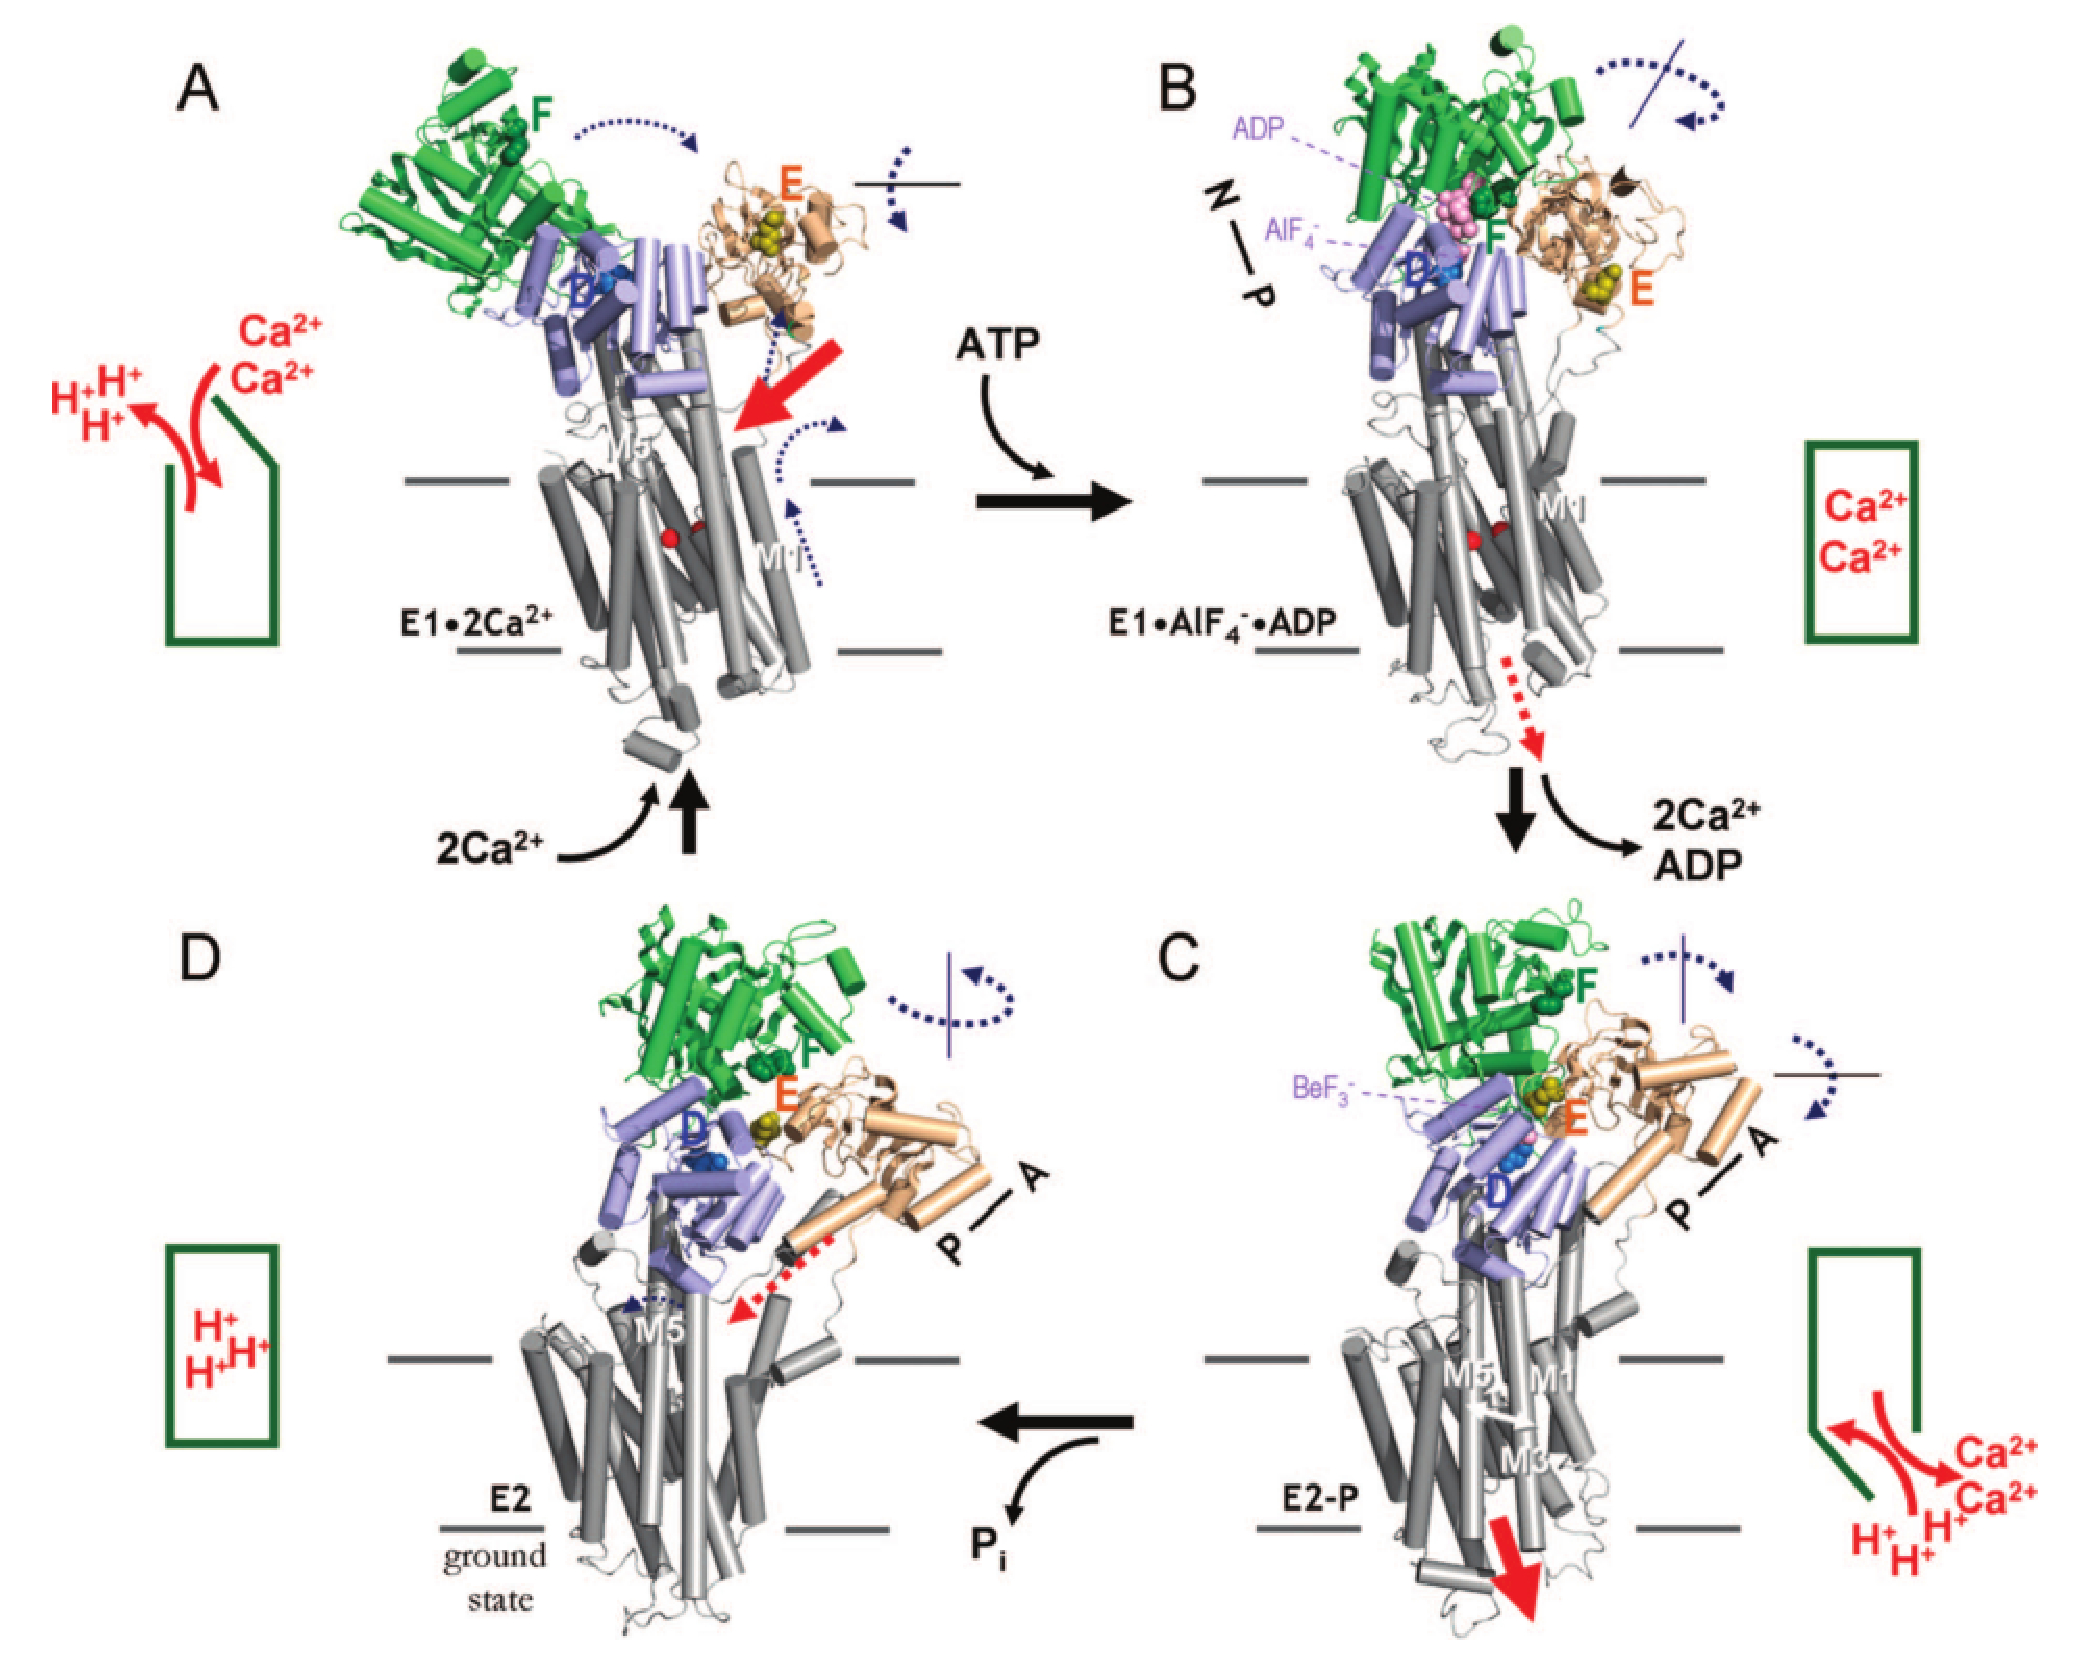
\includegraphics[height=8cm,
    angle=0]{./images/vangheluwe_serca.eps}}
\caption{Conformational changes of SERCA1a. Green rectangles represent
the sequential close and opening of SERCA \citep{Vangheluwe2006}}
\label{fig:vangheluwe_serca}
\end{figure}

Similar to Na/K-ATPase, \textcolor{red}{the SERCA pump has 2 major
conformations: E1 ($\Ca$-bound) and E2 ($\Ca$-free)} in which only E2 is coupled
to $\Ca$ transport~\citep{inesi1976}.  The equilibrium of
\begin{equation}
  \label{eq:1205}
  \ce{E1 <=> E2}
\end{equation}
is temperature-dependent and entropy-driven. In both forms, the
phosphorylated intermediate is formed in the presence of
$\Ca$. However, subsequent hydrolysis of the intermediate only occur
in the state E2.


In E1 form, the ion-transport sites face the cytosol and has high affinity for
$\Ca$. When $\Ca$ bound to the cytosolic side of the SERCA protein, it causes a
conformational change from E1 to E2, which is powered by the energy release from
the conversion of ATP to ADP. In E2 form, the ion-transport sites faces the
lumen of the ER and has a low affinity for $\Ca$. To model the balance of $\Ca$
leak vs. SERCA uptake, some models assume the backflux $\Ca$, i.e. pumping $\Ca$
from SR to cytoplasm \citep{shannon2000rms}. However, some experimentalists
believe that backflux doesn't happen at physiological condition, unless at very
high SR $\Ca$.
\begin{itemize}
\item models that assume back-flux: Sect.~\ref{sec:shannon-et-al}

\item models that ignore back-flux: Sect.~\ref{sec:tran-...-crampin}
\end{itemize}
It's believed that the $\Ca$ bound to SERCA pump doesn't contribute to the
calcium concentration in the cytosol nor the calcium concentratioin in the ER.
Thus, SERCA can serve as the calcium buffers. The amount of SERCA proteins is
quite large: 15-75 $\mu$mol/(L cyt.) in cardiac ventricular cell
\citep{bers2001ecc}. 


One important property of SERCA pump is that for every two $\Ca$
transport into the SR, 2-3 protons are counter transported, making SR
an electrogenic $\Ca/\H$
countertransporter~\citep{Yu1993,Hao1994,Peinelt2002}

A SERCA pump has gates on both sides: cytoplasmic gate and lumen SR
gate. A typical SERCA pump has 4 principal structures,
Fig.~\ref{fig:vangheluwe_serca}:
\begin{enumerate}
\item [[A]] $\Ca$ entry and bind to pump
  (\textcolor{red}{E2 $\rightarrow$ E1$\cdot 2\Ca$}) at two
  high-affinity $\Ca$-binding sites. The binding of 2 $\Ca$ is
  sequential, and cooperative. Even though $\Ca$ first meet gating
  residue Glu309 (part of site II), it cannot bind. this first $\Ca$
  need to proceeds to site I (binding at Asp800), where it fits
  better. This will induce a slight rotation of segment M6, and
  subsequently increase $\Ca$ affinity at site II, allowing $\Ca$ to
  bind to site II.

  2 $\Ca$ entry will release 2-3 protons ($\H$+) into the cytosol, and
  signal the phosphorylation to occur. This counter-transport can be
  incorporated into the model by (1) adding distinct $\H$ binding
  site~\citep{tran2009}.  The cytosolic access path to the binding
  sites, though, still open and bound $\Ca$ ions at Glu309 remain
  under constant attack by waters, and can be exchanged by other
  $\Ca$.

\item [[B]] ATP bind to the complex
  (\textcolor{red}{E1$\cdot 2\Ca$ $\rightarrow$ E1$\sim$ P
    phosphorylated state, presented by E1$\cdot$ADP$\cdot$\ce{AlF4-}
    structure}).
  In this process, ATP binds to Phe487 on N-domain. $\Mg$ and ATP
  (or aka MgATP) bridges the N-domain with P-domain at residue Asp351.
  The bending of the P-domain will close the cytosolic access path to
  the binding site II at Glu309. However, the pathway to lumen is not
  yet open, the SERCA pump is at an {\it occluded state},
  i.e. preventing further exchange of $\Ca$ from the cytosol.

\item [[C]] ATP is hydrolyzed, releasing energy for breaking the
  bridge N- and P-domain. The pumps change from high $\Ca$-affinity to
  low affinity form (\textcolor{red}{E1$\sim$P $\rightarrow$ E2-P}).
  The luminal exit pathway is formed, the rotation of segment M6 and
  large downward movement of M4 (Gluo309) distort the $\Ca$-binding
  sites, reducing the $\Ca$ affinity, which allows a quick release of
  $\Ca$ to the lumen SR. To stabilize the residues with empty $\Ca$,
  protons and water molecules from the lumen SR quickly bind to. This
  will switch the pump to E2-P state


\item [[D]] Dephosphorylation reaction
  (\textcolor{red}{E2-P $\rightarrow$ E2$\cdot$P}) start with the
  entrance of one water molecule to the phosphorylation site. The
  process lock the luminal gate for protons, releasing SERCA back to
  ground E2 state.
\end{enumerate}


\begin{figure}[hbt]
  \centerline{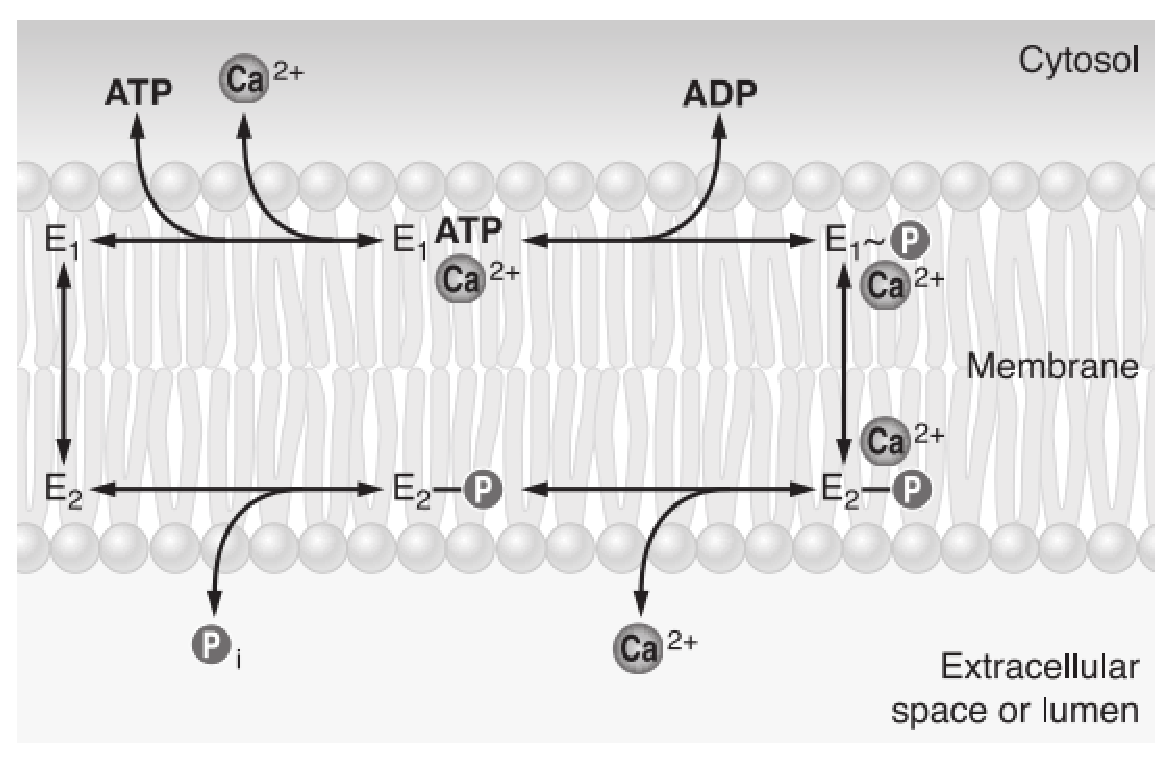
\includegraphics[height=5cm,
    angle=0]{./images/brini_CaATPase.eps}}
\caption{A simplified schematic diagram of $\Ca$-ATPase}
\label{fig:brini_CaATPase}
\end{figure}

\subsection{Calcium-uptake activity}
\label{sec:SERCA_Ca-affinity}

The $\Ca$ affinity of SERCA isoforms follow this relation: 2b $>$ 2a $>$ 1a $>$
2c $>$ 3, and turnover rates: 2b, c $<$ 2a $<$ 3b, b, c $<$ 1a
\citep{Lipskaia2013}. The $\Ca$ uptake activity of SERCA1a is similar to SERCA2a
\citep{dode2003}. The affinity for SERCA2a is $K_{0.5}=0.985 \muM$, yet with a
high turnover rate (ATP hydrolysis = 70 sec$^{-1}$) compared to SERCA2b
($K_{0.5}=0.508 \muM$ and ATP hydrolysis = 35 sec$^{-1}$) \citep{Dally2010}. The
$\Ca$ affinity of SERCA3a is 10-times lower than SERCA1a, yet with a rapid
turnover (around 100 sec$^{-1}$) \citep{dode2002}.

The $\Ca$ affinity of SERCA1 and SERCA2 is regulated by two intrinsic membrane
proteins: phospholamban (PLN) and sarcolipin (SLN) \citep{MacLennan2003,
MacLennan2003rsp}. SLN and PLN appear to bind to the same site, yet under
simulation of the ternary structure, PLN occupies the binding site, and SLN then
bind to the exposed side of PLN and SERCA. Both lower the apparent affinity for
$\Ca$ of SERCA1a and SERCA2a. NOTICE: SERCA3 isoforms lack PLN-binding domains
\citep{tada1996}.


\subsection{Models }
\label{sec:SERCA_models}

In many computational cell models, the SERCA pump is often modelled by a simple
Hill equation (Sect.\ref{sec:mich-ment-appr}), or by the Hill equation with
additional terms to account for modulation of ER calcium \citep{favre1996,
sneyd2003} (Sect.\ref{sec:serca_sneyd2003}). These models use the
phenomenologically based Michaelis-Menten description which typically involves
three parameters: $K_m, n$, and $v_{max}$ (Sect.~\ref{sec:mich-ment-appr}). This
class of models is often used in whole-cell modeling frameworks due to its
simplicity and computational efficiency.  These models work well in certain set
of physiological condition.
However, in pathological conditions when cell metabolism is compromised, e.g.
ischemia, those models don't work well due to the change in energetic production
in the cell that does affect the pumps behavior.

Some complex models consider the complex partial interactions with
various ionic species in the cytosol ($\mg$, \ce{K+}, and \ce{H+}), as
well as their interactions with cytosolic metabolites (MgATP, MgADP,
and Pi) (Sect.~\ref{sec:gould-et-al},
Sect.~\ref{sec:haynes-madveno-1987}). However, due to the complexity
of this kind of model, they're rarely used in whole cell modeling.

Another class of SERCA-pump model is the reversible model whose flux
is a function of cytosolic and lumincal $\Ca$ concentration (e.g.:
Sect.~\ref{sec:shannon-et-al}). However, as backflux has not been
observed {\it in vivo} in physiological conditions. There has been a
debate about the validity of such models. Recently, a newer class of
models have been proposed that doesn't produce back flux at normal
condition (Sect.~\ref{sec:tran-...-crampin}).

\subsection{SERCA isoforms in cardiac myocyte: expression level and subcellular
distribution}

SERCA2a is the major isoform, while SERCA2b is the minor cardiac isoform
\citep{Dally2010, vangheluwe2007}. In human heart, other isoforms have also been
detected, e.g. SERCA1a, SERCA2c and serveral SERCA3; yet their physiological
roles are not clear \citep{chemaly2013, Dally2006, Dally2009}.
\citep{summerfield2010} reported the role of SERCA1a upregulation in dilated
cardiomyopathy (DCM) in dogs.

To study subcellular distribution of SERCA pump in the cell, antibody to the
SERCA pump was used \citep{jorgensen1988} shown SERCA1 and SERCA2a are localized
in the longitudinal SR. In human, SERCA2a was restricted to the subsarcolemmal
compartment \citep{chemaly2013, greene2000, vangheluwe2007}. In mice, using
immunostaining isolated myocytes, SERCA2a was found distributed transversely
and longitudinally in the SR membrane, while SERCA2b focuses around the T-tubules
\citep{periasamy2001}. In human, SERCA3a is found close to the T-tubules and
intercalated disks; while SERCA3d is perinuclear and SERCA3f is subsarcolemmal
\citep{Dally2010, Dally2009}.
 

\citep{bers2001ecc} estimated about 15-70 $\mu$mol/(L cyt.) of SERCA proteins in
the cardiac myocytes. The total SERCA pumps/cell was estimated about 1,600,000
\citep{means2006}. In smooth muscle cells, it's estimated about 518 SERCAs/RyR
\citep{gomez-viquez2003}. Even though SERCA2b has a higher $\Ca$ affinity than
SERCA2a (Sect.\ref{sec:SERCA_Ca-affinity}), the expression level is much lower,
e.g. 8-10x increase in SERCA2b didn't reduce SERCA2a pump. This was explained by
the distinct in subcellular distribution between SERCA2b and SERCA2a.

Studies from mouse, rat and rabbit showed that SERCA expression level gradually
increases during development. This helps increase $\Ca$ uptake faster and thus
make the APD shorter \citep{periasamy2001}. The decrease in SERCA expression
levels have been found in several diseases, e.g. cardiac hypertrophy and heart
failure (review: \citep{lompre2010}). However, the study by
\citep{periasamy2001} showed that an increase in 2.5x is still in physiological
range. Restoration of SERCA2a expression by gene transfer can improve cardiac
functions \citep{Lipskaia2010, Kairouz2012} (review: \citep{chemaly2013}).  


\section{Regulatory factors}
\label{sec:SERCA_activity}

The activity of SERCA is controlled by various factors:
\begin{enumerate}
  \item $[\Ca]_i$ concentration (the higher the greater SERCA activity)
  \item SR $\Ca$ content (the higher, the slower SERCA activity)
  \item Recently, another regulator identified was sarcolipin (SLN)
  (Sect.\ref{sec:SLN_SERCA}).
  
  \item Natural inhibitory protein phospholamban \citep{tada1974} which
  enhances the SERCA uptake activity under the effect of $\beta$-adrenergic
  stimulation.
  
  \item In addition to common P-type inhibitors ($\La$ and othovanadate), SERCA
  pump can
be inhibited by specific inhibitors: {\bf thapsigargin}
(Sect.\ref{sec:thapsigargin_SERCA}), cyclopiazonic acid, and
2,5-di(t-butyl)hydroquinone. 
   
\end{enumerate}

Changes in SERCA activity can affect amplitude of systolic $\Ca$ transient and
then cardiac contractility; thus has been linked to pathological conditions of
the heart. However, the affect of change in SERCA activity to SR $\Ca$ content
has been controversy.  

There are abundant of evidences that SERCA activity is decreased in heart
failure (HF)\citep{hasenfuss1994, hobai2001}. There are efforts to treat HF
using viral transfer of SERCA genes to improve SERCA
concentration\citep{kawase2011}. So, can we study the effect of SERCA by
knocking out partially SERCA pump?
\begin{itemize}
  \item completely knockout is embryonically lethal \citep{periasamy1999}
  \item recent techniques allow reducing SERCA activity to less than 5\% of
  control, but animals continue to live for 6-8 weeks \citep{andersson2009}.  
\end{itemize}

Recently, \citep{bode2011}, using thapsigargin (1$\muM$) on rat ventricular
myocytes, has shown that change in SERCA pump has modest effect on SR $\Ca$
content.

% \subsection{Inhibitors (PLN, SLN)}
% \label{sec:inhibitors-pln-sln}

\subsection{Phospholamban (PLN, PLB)}
\label{sec:phospholamban}
\label{sec:PLN_SERCA}

Phospholamban (PLN, PLB)  is a 52-amino acid integral membrane protein that
regulates the SERCA-Ca2+ATPase pump (Sect.\ref{sec:SERCA_pump}) in cardiac
muscle and skeletal muscle cells. Phospholamban is not expressed in neuron.

Phospholamban (PLN) is the endogenous modulator that inhibits the activity of
SERCA pumps (SERCA1a, SERCA2a, SERCA2b), but not SERCA3 \citep{james1989}.
Mutagenesis studies showed that SERCA sequence essential for PLN-regulation is
Lys$^{397}$-Asp Acid-Asp Acid-Lys-Pro-Val$^{402}$ \citep{toyofuku1994} which is
not found in SERCA3.

\begin{itemize}
  \item unphosphorylated form of PLN inhibit SERCA
  
  \item phosphorylated form of PLN cannot inhibit SERCA as they disrupt the
  cytoplasmic interaction with SERCA
\citep{koss1996, kadambi1997, MacLennan2003}, i.e. the inhibition
  is removed, i.e. enable $\Ca$ uptake is faster leading to shorter intervals
  between contraction. 
  
  PLN can be phosphorylated by different kinases.
  
  \begin{enumerate}
    \item  PKA (cAMP/cGMP-dependent protein kinase)
  (Sect.\ref{sec:PKA}).

    \item  protein kinase C (PKC, Sect.\ref{sec:PKC})
    
    \item  Ca/Calmodulin-kinase II (CaMKII)
  \end{enumerate}
  at the site Ser$^{16}$, Ser$^{10}$, and Thr$^{17}$, respectively.
\end{itemize}

This interaction is importance because during heart failure condition, when
SERCA pump level has already decreased (50\%) This, as the result, remove the
inhibiting effect of PLN, making SERCA activity increases. The phosphorylation
of PLN substantially contribute to the {\it inotropic} (enhanced contraction),
and lusitropic (enhance relaxation rate).
So, the condition can be more severed with the inhibition of dephosphorylated
PLN (lower $\Ca$ affinity and $v_\max$ of SERCA pump) \citep{dash2001}.
 
\begin{framed}
During $\beta$-adrenergic stimulations, at least 2 sites of PLN are
phosphorylated {\it in vivo}: Ser16 by cAMP-dependent protein kinase,
and Thr17 by $\Ca$/calmodulin-dependent kinase II (CaMKII). 

Protein phosphatases can dephosphorylate PLN. So, phosphorylation and
dephosphorylation of PLN can regulates SERCA activity in response to different
stimuli.
\end{framed}

PLN lowers the $\Ca$ affinity of SERCA and thus holds the pumps at E2
conformation (Sect.\ref{sec:SERCA_conformations}). Cytosolic PLN interacts with residues
in the N-domain of the pump.  Unphosphorylated (or dephosphorylated)
phospholamban can inhibit SERCA1 and SERCA2, by decreasing its affinity to
calcium.


\begin{framed}

There's a kinase sensitive to $\Ca$, from the SR side, that is activated upon
the store depletion to phosphorylate Ser$^{16}$ in the cytoplasmic domain of
PLN, thereby stimulating the refilling of SR \citep{bhogal1998}. Hower, this
raised the question how this kinase and protein kinase A compete to the same
binding site.
\end{framed}

To study the colocalization between PLN and SERCA at different concentration of
$[\Ca]_i$, FRET imaging technique was used \citep{bidwell2011} where PLN bound
to yellow fluroescent protein (YFP) and SERCA bound to Cerulean. 


\subsection{Thapsigargin}
\label{sec:thapsigargin_SERCA}

Thapsigargin (TG) is the most characterized and popular inhibitor to SERCA. Its
affinity to SERCA pump is very high: $K_d$ in the sub-nanomolar range have been
measured. It binds stoichiometrically to F256 of the segment M3, locking the
pumps to an irreversible inactive state, i.e. inhibit permanently. 1$\mu$M
thapsigargin can inhibit partially to completely SERCA, when it was added
together with $\MgATP$~\citep{yano2000} and depending on the duration
70-130s\citep{bode2011}.


\begin{framed}
  Ser16 phosphorylation is a prerequisite for Thr17 phosphorylation
  during $\beta$-adrenergic stimulation. However, under pathological
  conditions, Thr17 phosphorylation independent from Ser16 was also
  observed.
\end{framed}

All SERCA isoforms are potently and selectively inhibited by thapsigargin (TG)
\citep{lytton1991}. \textcolor{red}{Thapsigargin binds to a site in TMS3 and locks irreversibly the
pumps} \citep{sagara1992}.

\begin{framed}
  A reduced SERCA2a activity, at least, partially diminished cardiac
  contractility function. So, enhancing SERCA2a pumps seem an
  appealing strategy to reverse the progression of heart failure. 
\end{framed}

\subsection{Sarcolipin}
\label{sec:SLN_SERCA}

Sarcolipin (SLN) expressed dominantly in fast-twitch skeletal muscle and inhibit
SERCA upon activation. SLN is co-expressed with SERCA2a, and PLN in the atria (but not
in ventricle) and in slow-twitch skeletal muscle~\citep{Vangheluwe2009}. SLN
activity is controled  by $[\Ca]_i$. So the dual  effect is that at low
$[\Ca]_i$, sarcolipin decrease SERCA acitivy yet stimulates SERCA uptake rate
($v_\max$) at saturating $[\Ca]_i$  \citep{odermatt1997}.


\subsection{Nmoc-DBHQ (synthesis, reversible)}

\citep{Rossi1997} used Nmoc-DBHQ as a 'caged' agent to inhibit SERCA when needed
by using photolysis. 

\section{Michaelis-Menten approach}
\label{sec:mich-ment-appr}


The phenomenologically simple model based on Michaelis-Menten
description has the equation of familiar form (producing rectangular
hyperbola shape)
\begin{equation}
  \label{eq:976}
  J_\serca = \frac{v_{max}}{1+(K_m/[S])^n} = 
  \frac{v_{max}[S]^n}{[S]^n+(K_m)^n} 
\end{equation}
with $v_{max}$ is the maximum velocity, $n$ is the Hill
coefficient. $K_m$ is the Michaelis-Menten constant, [S] is the
substrate concentration, and possibly including other terms like [I]
(inhibitor concentration) and $K_i$ (inhibitor constant).

This approach was used in~\citep{kanazawa1971, bassani1994rir}.

The main disadvantage of this approach is that it works well for a
certain limited set of conditions only (those was used to fit the
parameters). In vivo, $K_m, K_i$ are not constant but functions of
other reactants. So, the model contains an implicit assumption of a
single rate-limiting step, i.e. the reactions were treated as
equilibrium or quasi-equilibria.



% \subsection{Bassani et al. (1994)}
% \label{sec:bassani-et-al}
\subsection{Klein - \ldots - Schneider (1991): Ca-cyto dependent}
\label{sec:SERCA-Michaelis-Menten_Klein-Schneider-1991}

The steady-state activity of the SERCA pump is assumed to be dependent upon
calcium in the cytosol only (read sect.~\ref{sec:indo-1}). 

In addition, the number of $\Ca$-binding sites is $n$, with fast binding is
assumed (or infinitely co-operative binding).
% This method is based on the classic approach model the pumps
% (Sect.~\ref{sec:mich-ment-appr}). However, it use a non-unitary Hill
% coefficient $n$
The steady-state transport rate (v) is assumed simply proportional to the
fraction of pump units having $n$ bound calcium ions, and can be formularized as
\begin{equation}
  \label{eq:962}
\begin{split}
  J_\serca &= v_{max}\frac{([\Ca]_i)^n}{([\Ca]_i)^n+(K_m)^n} \\
  &= v_{max}\frac{1}{1+(K_m/[\Ca]_i)^n}
\end{split}
\end{equation}
with $K_m = 184$nM, $v_{max}=208\mu$M/s, $n=3.98$. 
NOTE: $K=(K_m)^n$  is the $n$-th order dissociation constant of calcium binding.

At the resting level, where $([\Ca]_i)^n << K$, then the rate $v=J_\serca$
is $v_\max \times (([\Ca]_i)^n/K)$.
In cell, the flux is balanced by a non-pump-mediated leak flux component.

% To provide the best fit to equilibrium rates for the interaction of SR Ca-ATPase
% with $\Ca$ in cardiac cells.

Other whole-cell models use the similar approach to model SERCA
pump~\citep{klein1991,sipido1991,
  balke1994,wier1994lce,luo1994dmc_a,luo1994dmc_b}.




\subsection{Balke et al. (1994)}
\label{sec:balke-et-al}

~\citep{balke1994} use classic Hill equation to model SR-ATPase pump
\begin{equation}
  \label{eq:1434}
  J_\serca = v_\serca \frac{[\Ca]^\etaserca}{[\Ca]^\etaserca+K_\serca^\etaserca}
\end{equation}
with $v_\serca = 0.21\pm0.04$ mM/s, $K_\serca=0.28\pm 0.04\mu$M,
$\etaserca=1$. 

\subsection{Snyder et al. (2000)}

Using Henri/Michaelis-Menten sequence, which accounts for feedback from the
product ($[\Ca]_\nsr$) of the reaction (SR uptake), the rate of $\Ca$ uptake is
given by the second-order reversible Michaelis-Menten kinetics
(Sect.\ref{sec:snyder_2000})
\begin{equation}
J_\serca = v_{\max, \serca} \frac{\left([\Ca]_\myo^2 -
(\frac{[\Ca]_\nsr}{7000})^2\right)}{\left(K_{m,\serca}^2 + [\Ca]_\myo^2 -
(\frac{[\Ca]_\nsr}{7000})^2\right)}
\end{equation}
It's better than the two above formula as it consider both $[\Ca]_\myo$ and
$[\Ca]_\jsr$ dependent. The formula was taken into account the thermodynamically
limited gradient of 7000 that SERCA pump can produce between SR and cytosol
\citep{shannon1997}.  

In a typical SERCA uptake study, oxaloacetate anion is used to empty $\Ca$ in
the SR, then the equation is reduced to the familiar form cited in the above studies
\begin{equation}
J_\serca = \frac{v_{\max,\serca}\left( [\Ca]_\myo \right)^2}{(K_m)^2 + \left(
[\Ca]_\myo \right)^2}
\end{equation}

\subsection{Sneyd et al. (2003)}
\label{sec:serca_sneyd2003}

\citep{sneyd2003}

\section{Mikanose et al. (1973)}
\label{sec:mikanose-et-al}

In E1-E2 model, the SERCA pump is assumed to have 2 $\Ca$ binding
sites, with affinities for $\Ca$ depends on their orientation. The
binding sites have much higher affinity when it faces the cytosol,
than when they face the lumen SR. 



\section{Meis-Vianna (1979)}
\label{sec:meis-vianna-1979}

~\citep{deMeis1979}

\section{Inesi et al. (1980)}
\label{sec:inesi-et-al}

~\citep{inesi1980} modeled with 6 steps $\Ca$-ATPase cycle. 


\section{Gould et al. (1986)}
\label{sec:gould-et-al}

The $\Ca+\mg$-activated ATPase (ATP phosphohydrolase, EC 3.6.1.3) of
SR exhibits a complex kinetics of activation w.r.t ATP.
\begin{enumerate}
\item ATPase activity is pH-dependent
\item ATPase activity is activated by low concentration $\Ca$ ($\mu M$
  range), and is inhibited by high concentration of $\Ca$ (mM range)
\end{enumerate}
The ATPase is postulated to exist in 2 conformations: (E1) with high
affinity to $\Ca$ and MgATP; (E2) with low affinity to $\Ca$ and
MgATP. The effect of ATP on E1-E2 transition follow a consequence of
different binding constant of ATP for the two forms, i.e. the
equilibrium constant between E1-E2 and E1ATP-E2ATP will not be equal,
and forward/backward rates between E1 and E2 are unequal with those
between E1ATP and E2ATP.

The binding of $\Ca$ to ATPase, in the absence of ATP, show a slow
conformation step from E1 to E1'Ca, compared to when having
ATP. Specifically, the rate constant of the conformation step is 180
s$^{-1}$ (with ATP), and 12 s$^{-1}$ (absence ATP). 

\begin{figure}[hbt]
  \centerline{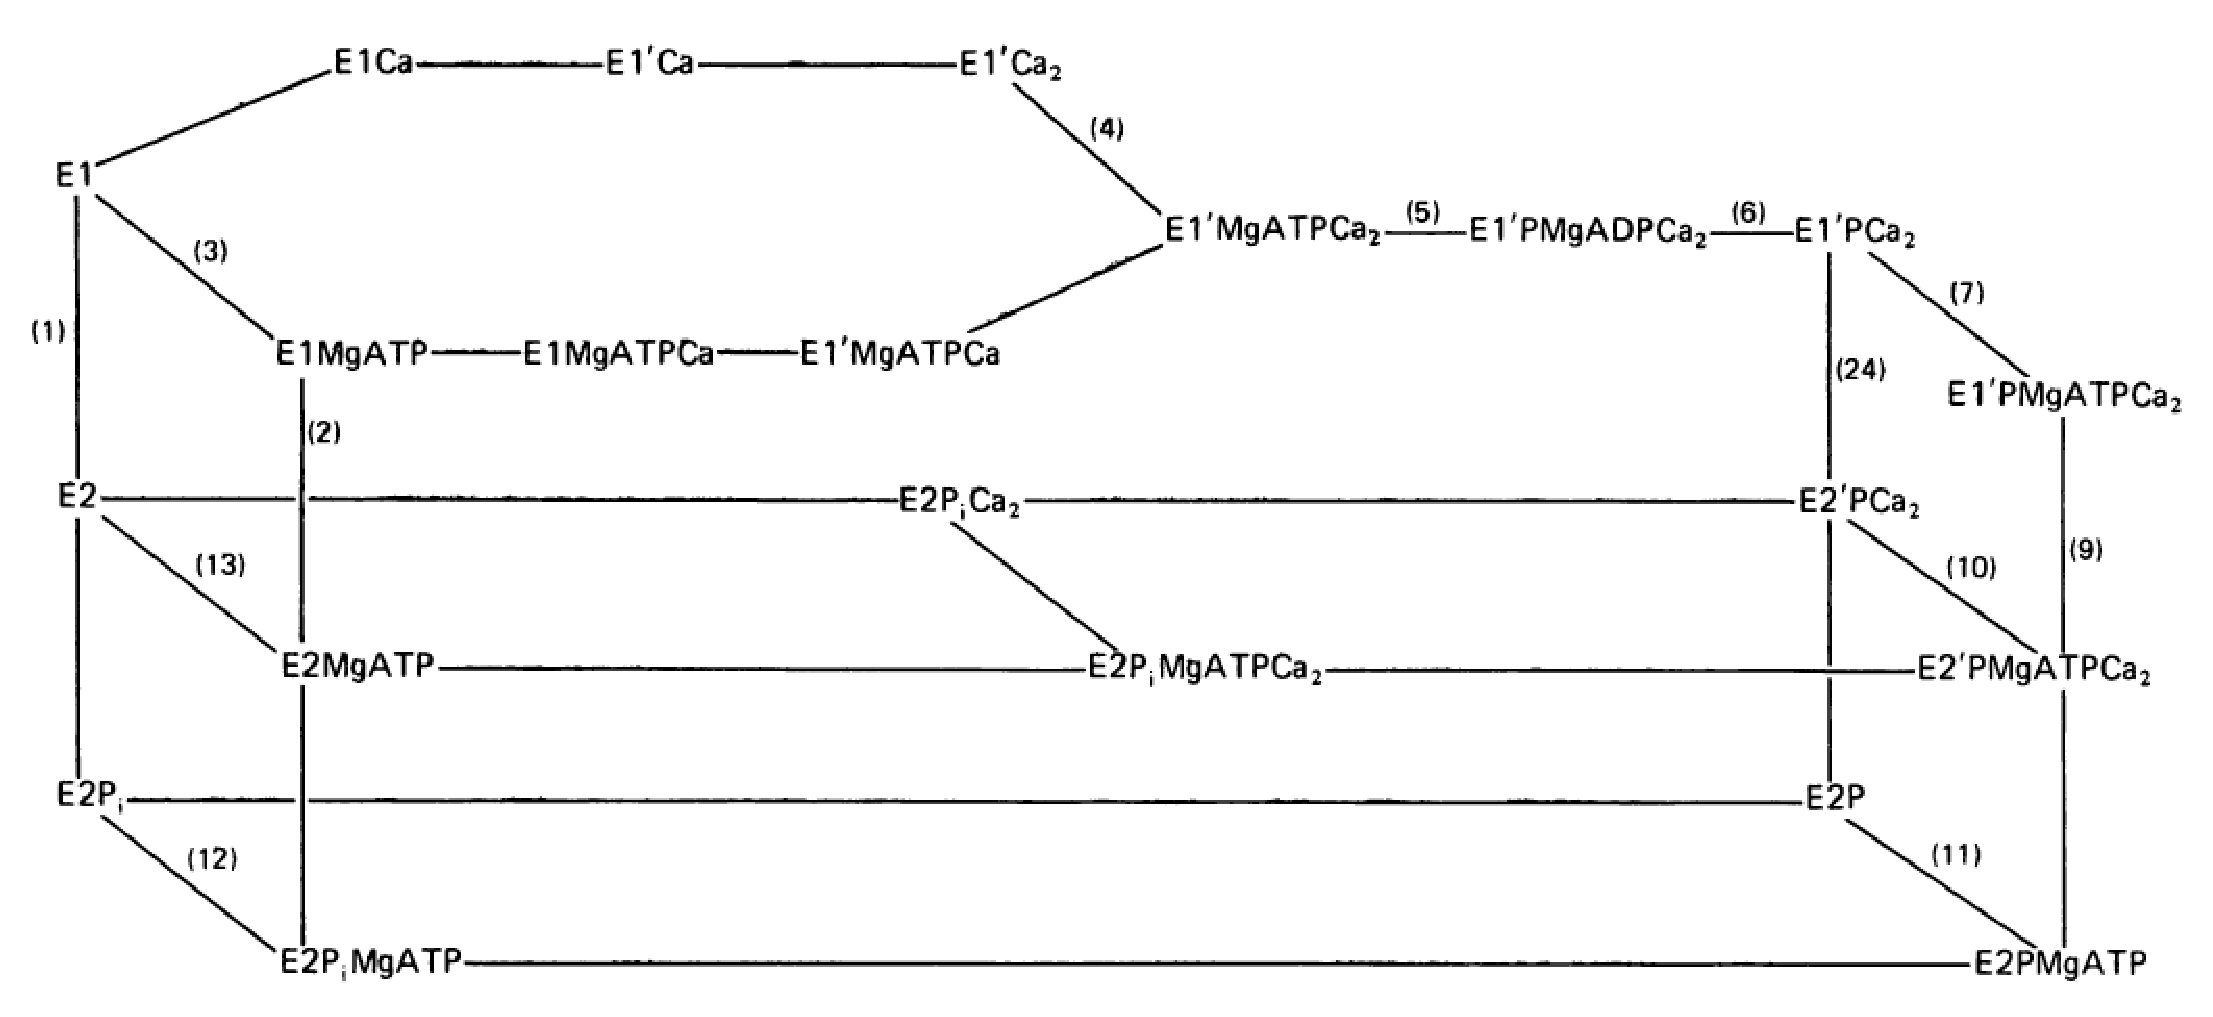
\includegraphics[height=5cm,
    angle=0]{./images/serca_scheme.eps}}
\caption{Reaction mechanism of SERCA}
\label{fig:serca_gould}
\end{figure}

\begin{figure}[hbt]
  \centerline{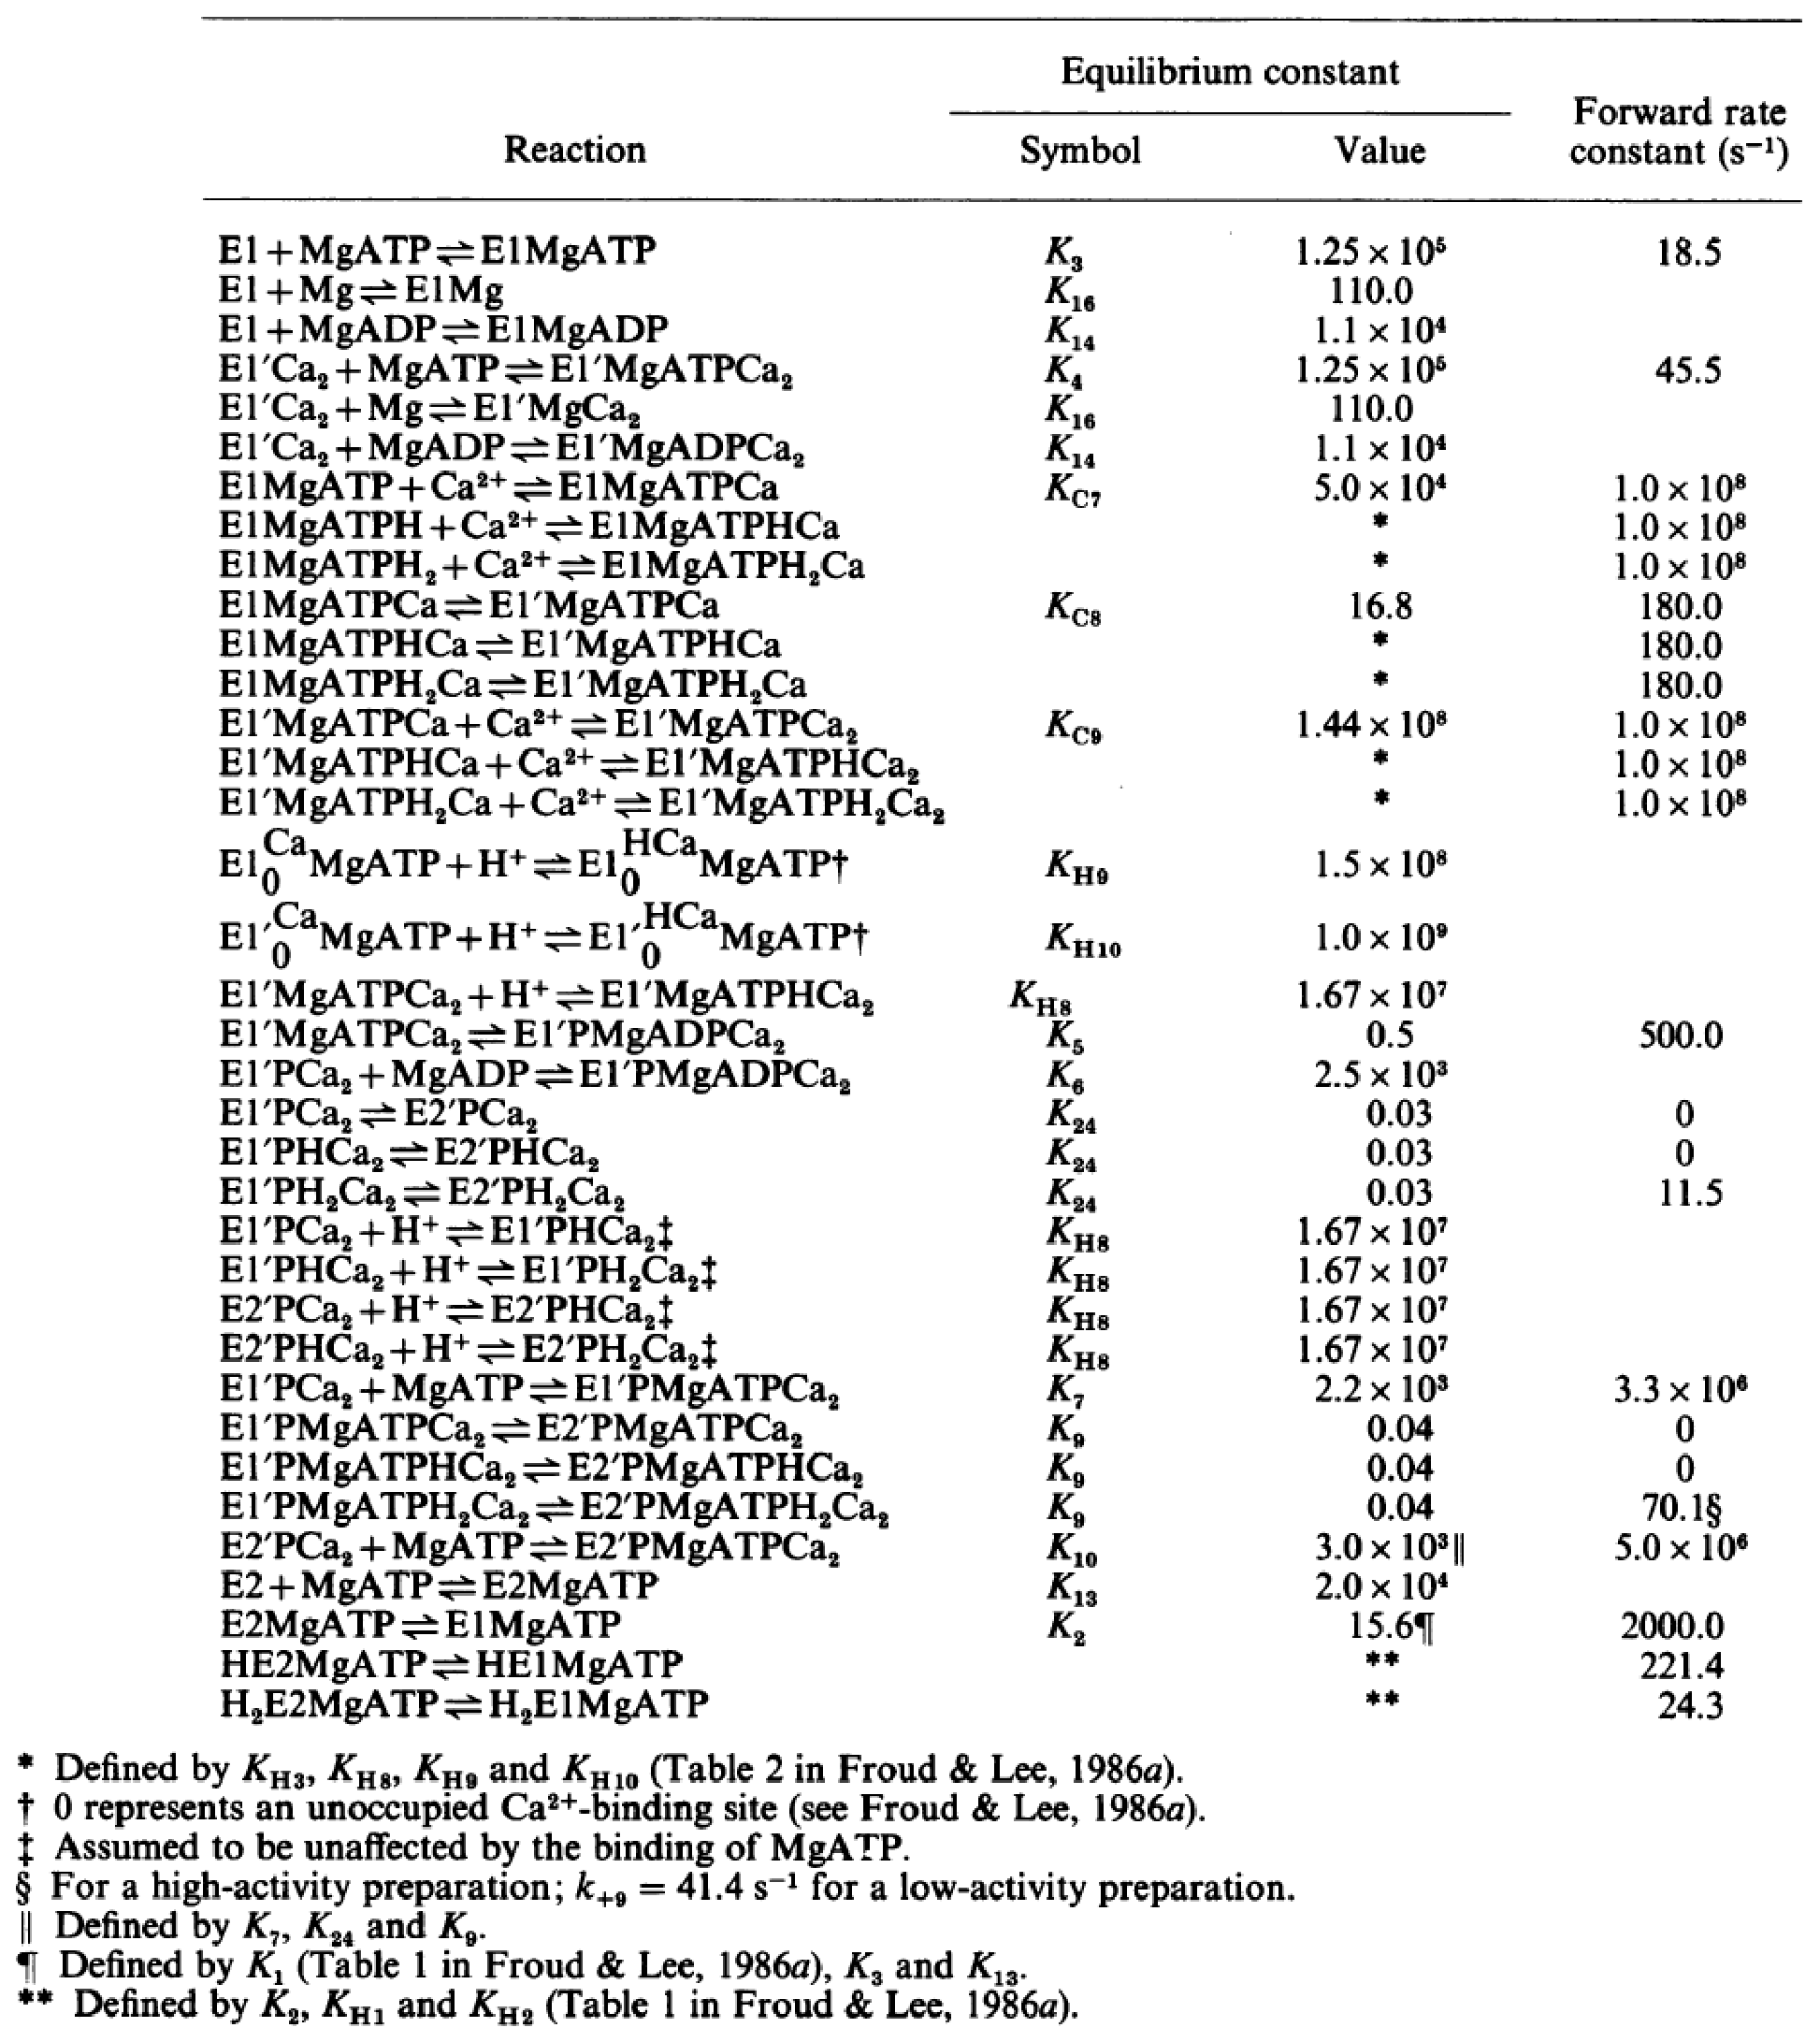
\includegraphics[height=5cm,
    angle=0]{./images/gould_serca_reaction.eps}}
\caption{kinetics reactions and parameters obtained at 25$^\circ$C}
\label{fig:kinetic_param_serca_gould}
\end{figure}

\begin{figure}[hbt]
  \centerline{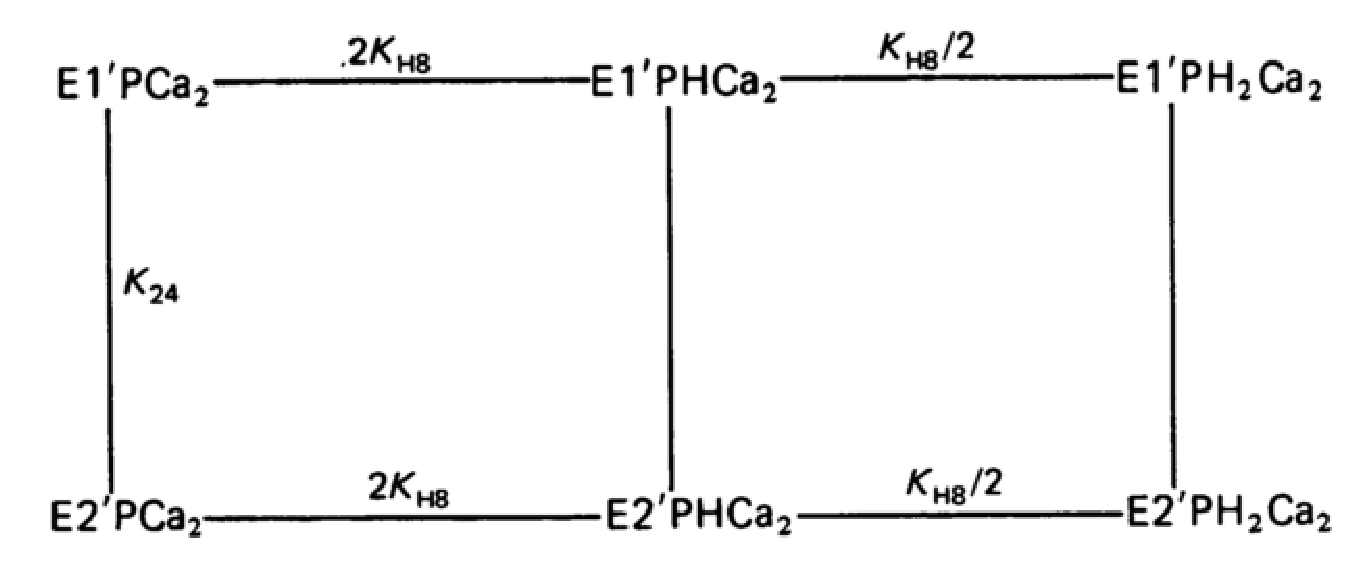
\includegraphics[height=3cm,
    angle=0]{./images/gould_effect_pH.eps}}
 \caption{Effect of pH on E1'PCa$_2$-E2'PCa$_2$ transition}
\label{fig:gould_effect_pH}
\end{figure}


\section{Haynes-Madveno (1987)}
\label{sec:haynes-madveno-1987}


In this approach, they estimates the rate and equilibrium constants
and seeks to generate the enzymatic behavior. The model utilized
\begin{enumerate}
\item cooperativity of (one or two) $\Ca$ binding (positive) and
  proton H$^+$ binding
\item ``grand partition function'' involve intrinsic binding constants
  and interaction energies and cooperativity parameters. 
\end{enumerate}

To reduce the computational demands, 5 of the 18 states was assumed to
be in rapid equilibrium, and the remaining was solved using matrix
method. 

A further simplification was that 5 steps in the cycle were
irreversible, i.e. the backward rate constant of zero. 

\section{Shannon et al. (1997, 1998, 2000, 2002)}
\label{sec:shannon-et-al}

Whole-cell models typically use classic Hill equation to model the SERCA pump
and a non-pump-mediated leak flux component. This classic approach doesn't take
into account the luminal calcium $[\Ca]_{sr}$ (i.e. $[\Ca]_\jsr,[\Ca]_\nsr$).
The reason that Hill equation is not a good option is given below

\begin{framed}
  At rest, when total concentration of $[\Ca]_\nsr$ is relatively
  constant, the SERCA pump rate must be about the same as the leak,
  but in opposite direction. However, using Hill equation for a SERCA
  pump with $K_m=0.2-0.6\mu M$, the resting steady-state calcium pump
  flux still at the magnitude of about 1/5 of the maximum SERCA pump
  rate. To maintain a constant SR load at rest, this requires a
  relatively large leak which unnecessarily deplete the cell energetic
  phosphate.  
  
  Furthermore, it has been shown that the maximum $[\Ca]_\nsr$ is relatively
  independent of  SERCA pump velocity~\citep{ginsburg1998}. It suggests that SR 
  calcium leak must be very low. In fact, a measurement in intact  cells shown a
  resting value of leak flux 0.32$\mu$M/s, i.e. 100x  lower than the pump-leak
  balance at resting $[\Ca]_i$ using Hill equation as mentioned above. The
  measured value agrees with SR calcium leak rate, at resting, between
  0.2-0.8$\mu$M/s~\citep{cheng1993cse}. So, a proper model for SERCA pump should
  be non-Hill equation. 
\end{framed}

Shannel et al. proposed a model for SERCA pump with forward and backward rates,
Fig.\ref{fig:Shannon2000_backflux}. Backward rate increases the SR is filled.
Thus, a net balance of SR fluxes occur when lumenal $[\Ca] \sim 7000$ times the
sarcoplasmic $[\Ca]$ (i.e.
$[\Ca]_myo=0.1\muM$, $[\Ca]_\nsr=700\muM$). Here, 60\% of SR leak is modeled via
RyR, and 40\% is via backflux.

\begin{figure}[hbt]
  \centerline{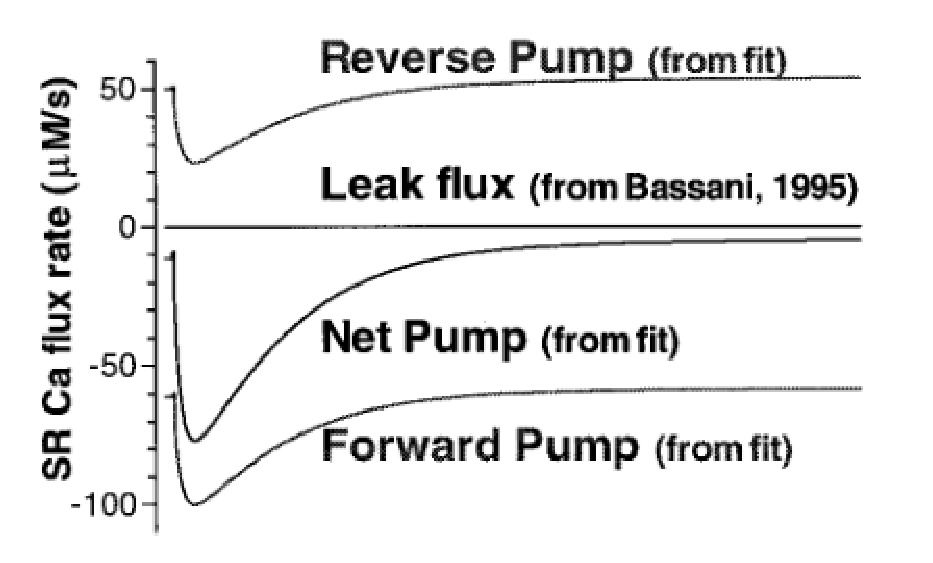
\includegraphics[height=5cm,
    angle=0]{./images/Shannon2000_backflux.eps}}
  \caption{Backflux in SERCA pump model}
  \label{fig:Shannon2000_backflux}
\end{figure}

A variation of Shannon model has been incorporated into different whole-cell
models: in rats \citep{snyder2000mmc} (Sect.\ref{sec:snyder_2000}), in
integrated cell model to study interval-force relation \citep{rice2001mch}.


\subsection{Hypothesis analysis}
\label{sec:hypothesis-analysis-10}

With small leak flux,
\textcolor{red}{the authors hypothesized that there is a backflux to
  account for the leak, though via SERCA
  pump}~\citep{shannon1998,shannon2000rms,shannon2002}.


\begin{figure}[hbt]
  \centerline{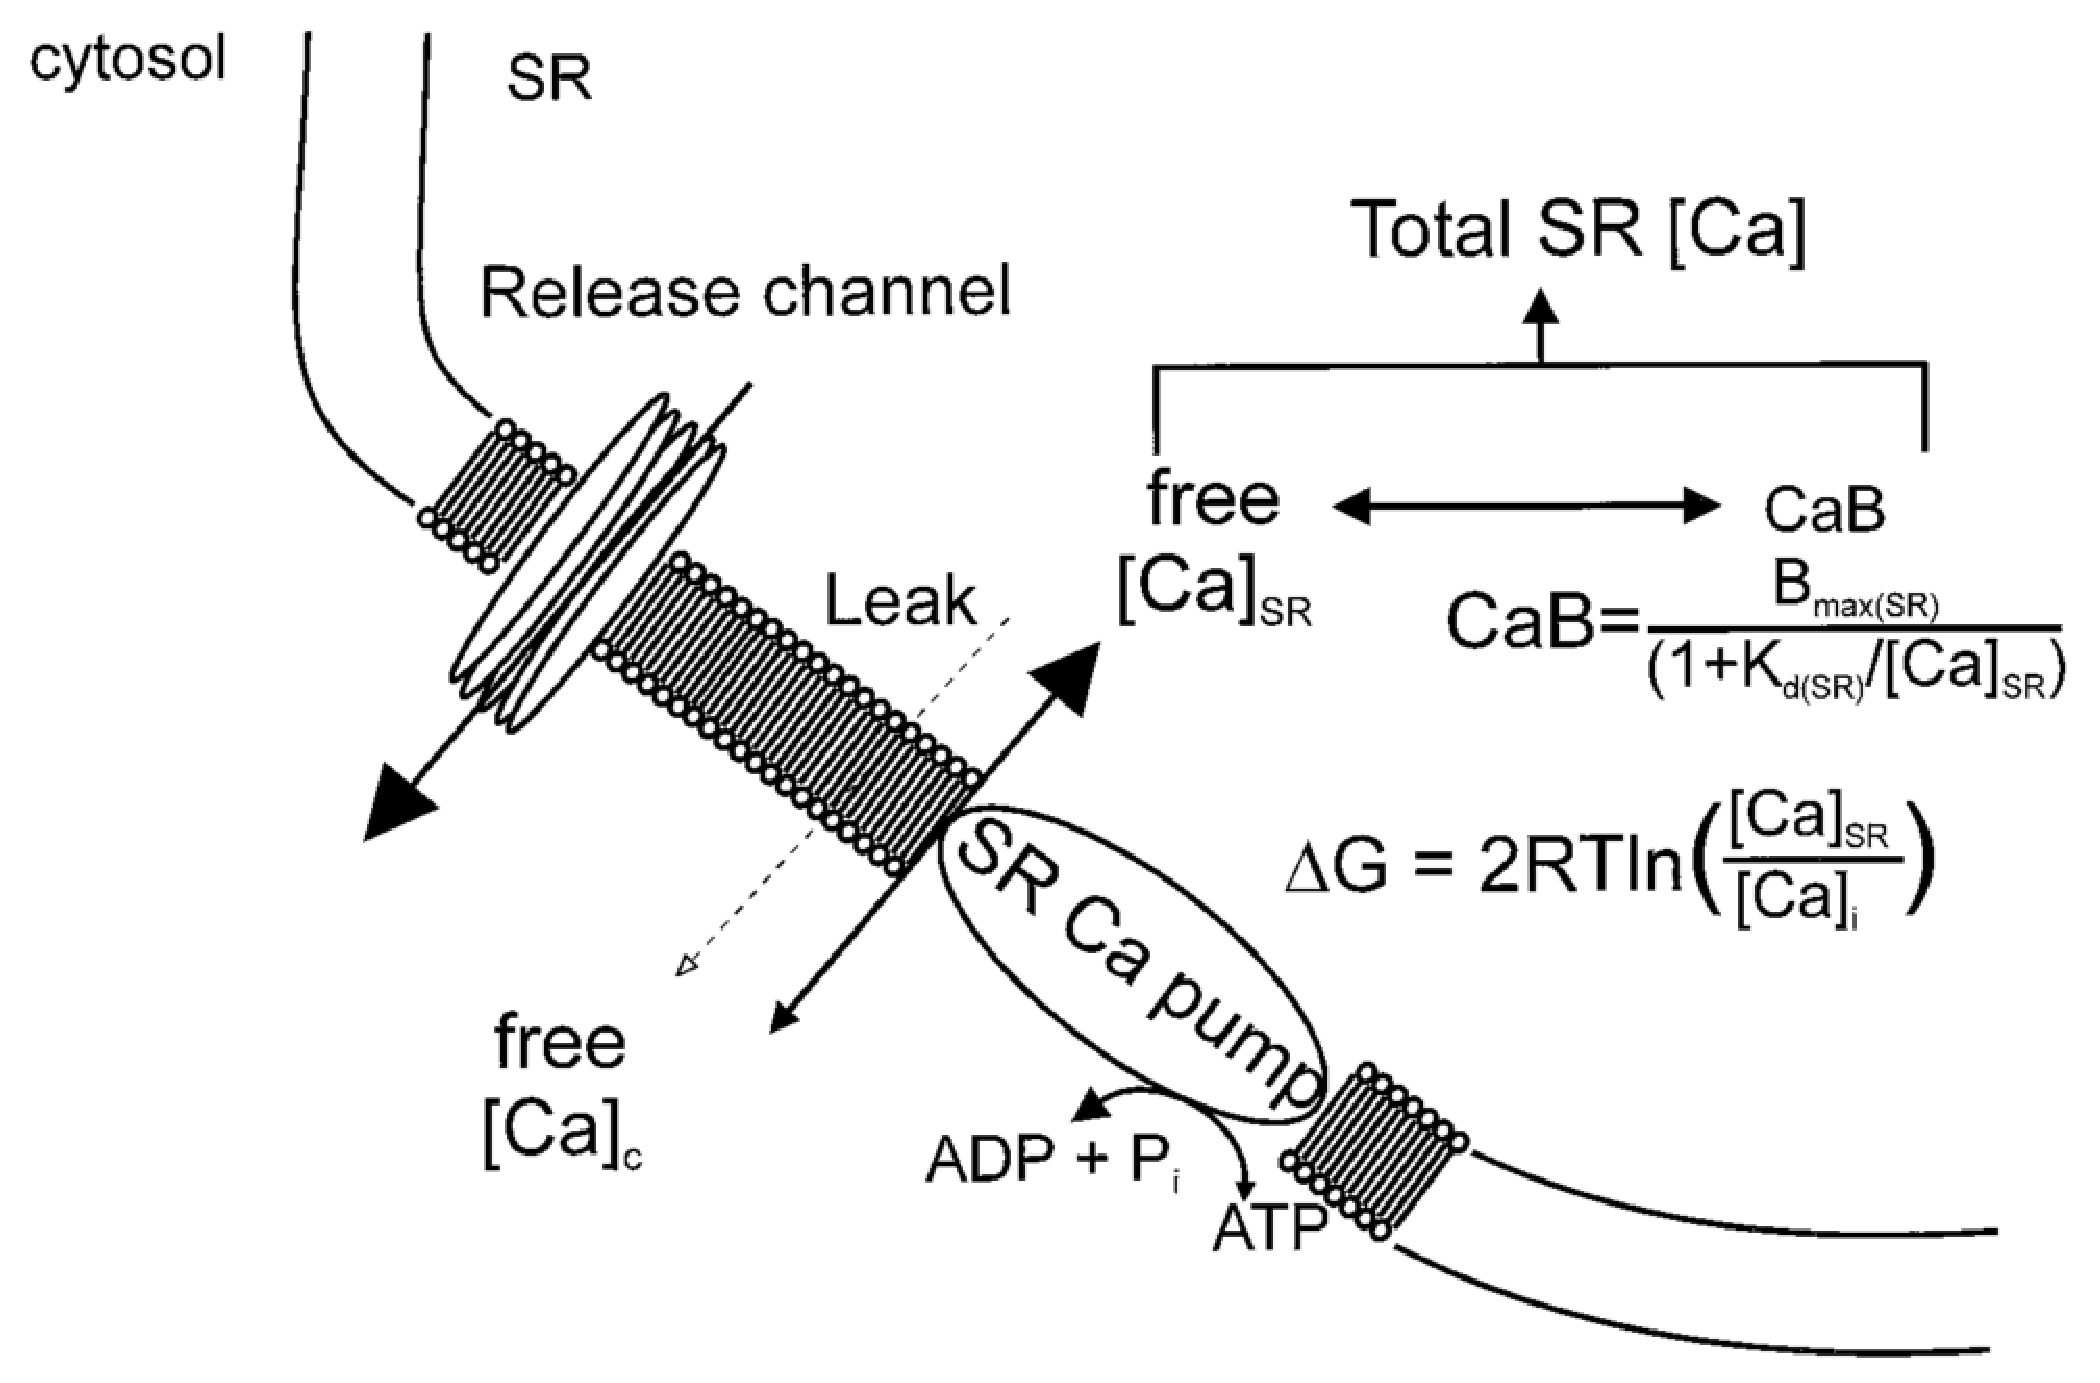
\includegraphics[height=5cm,
    angle=0]{./images/shannon_serca.eps}}
\caption{The schematic diagram for the SR show a passive leak, an
  active forward and reversal reverse mode of the SERCA}
\label{fig:shannon_serca}
\end{figure}


They proposed a thermodynamics model in which the gradient is derived
from the free energy available from cytosolic ATP ($\Delta G_{SRCa}$),
Fig.~\ref{fig:shannon_serca}, when the pump is at steady state
\begin{equation}
  \label{eq:1025}
  \Delta G_{\text{SRCa}} = z_\Ca RT \ln K_{eq}=z_\Ca RT \ln\left(\frac{[\Ca]_\sr}{[\Ca]_\myo}\right)
\end{equation}
with $K_{eq}=7000$~\citep{shannon1997}.

which drives the pump in forward mode. The idea of {\bf ``backflux''}
is that the accumulated $[\Ca]_\nsr$ also slow the net SERCA pump
rate, and nearly stopping it, at resting, through the pump in the
direction from SR to cytosol, which in turns reproduce ATP from ADP +
P$_i$. This reproduction of ATP will result in much less energy use,
compared to the less-efficient pump-leak balance (described by Hill
equation). This has been demonstrated in some experiments, yet it's
now clear how this works in intact myocardial cells.


\subsection{Mathematical model}
\label{sec:mathematical-model-15}

The calcium-bound to indo-1 was calculated using eq.~(\ref{eq:977}).
Global cytosolic concentration change is the change in free calcium,
calcium bound to ligands (L), and the contribution from other fluxes.
\begin{equation}
  \label{eq:982}
  \frac{d[\Ca]_{tot}}{dt} = \frac{d[\Ca]_i}{dt}  + .... + J_\serca + ...
\end{equation}
Thus, the flux of calcium via SR $J_{sr}$ is
\begin{equation}
  \label{eq:981}
  J_{sr} = \frac{d[\Ca]_{tot}}{dt} - (\frac{d[\Ca]_i}{dt} +
  \frac{d[\Ca\cdot L]_{tot}}{dt} + J_\ncx + J_{I_{Ca}} + J_{mito} + J_{SLpump})
\end{equation}
$J_{I_{Ca}}$ was converted to $\mu M/s$ using capacitance/volume ratio
of 6.44pF/pL cytosol~\citep{sipido1991}.

There are total 8 different ligands considered in the model
\begin{equation}
  \label{eq:983}
  \frac{d[\Ca\cdot L]_{tot}}{dt}= \sum^8_{i=1} \frac{d[\Ca\cdot L_i]}{dt}
\end{equation}
\begin{figure}[hbt]
  \centerline{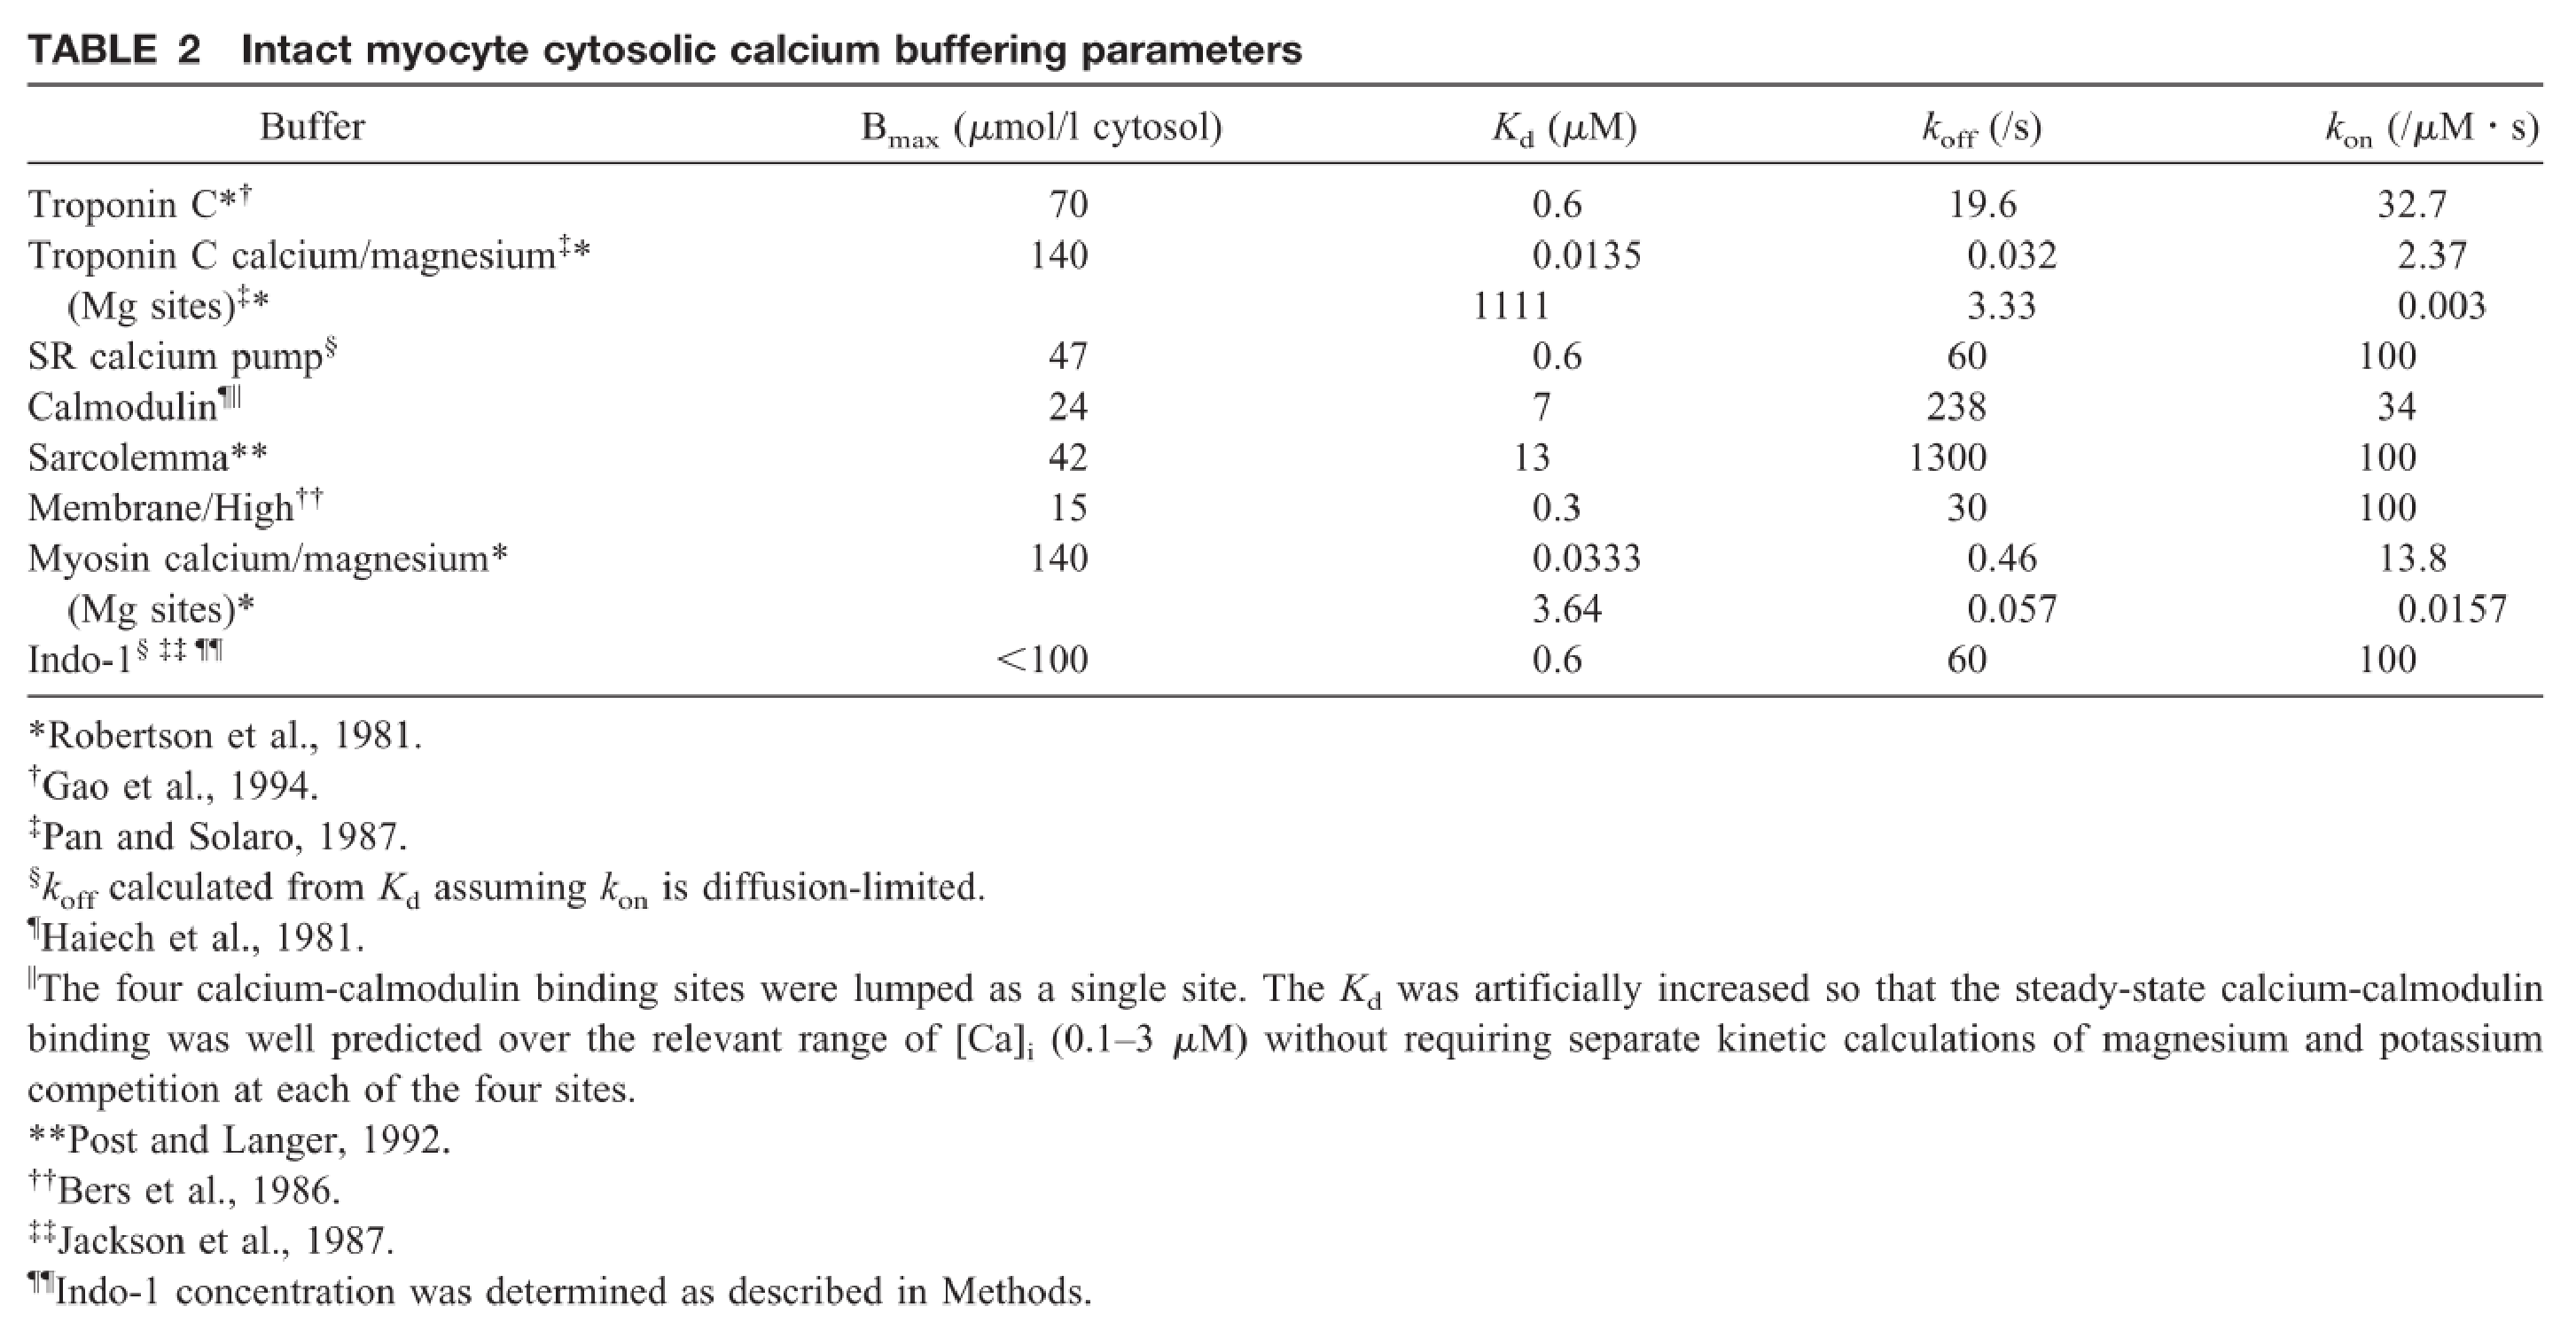
\includegraphics[height=5cm,
    angle=0]{./images/shannon_ligands.eps}}
\caption{Buffering parameters for 8 different ligands}
\label{fig:shannon_buffers}
\end{figure}

$J_{sr}$ composes of 3 components: $J_{pump}$ the net pump flux via
SERCA, $J_\rel$ (or $J_\ryr$), and $J_\leak$.
\begin{equation}
  \label{eq:984}
  J_{sr} = J_\serca + J_\ryr + J_\leak
\end{equation}
In their experiment, $J_\ryr=0$ as the data were measured at late part
of $[\Ca]_i$ transient when SR release via RyR is over. Finally, the
equation that incorporate both SERCA pump and leak is given
\begin{equation}
  \label{eq:985}
  J_{sr} = \frac{v_{maxf}\left( \frac{[\Ca]_i}{K_{mf}} \right)^{Hf} -
    v_{maxr}\left( \frac{[\Ca]_{sr}}{K_{mr}} \right)^{Hr}  }{1+ \left(
      \frac{[\Ca]_{i}}{K_{mf}} \right)^{Hf} + \left( \frac{[\Ca]_{sr}}{K_{mr}} \right)^{Hr}} +
  k([\Ca]_{sr} - [\Ca]_i)
\end{equation}
which can be broken into the leak flux, the forward and backward
fluxes
\begin{eqnarray}
  \label{eq:986}
  J_\leak &&=   k([\Ca]_{sr} - [\Ca]_i)\\
  J_{serca,f} &&= 
  \frac{v_{maxf}\left( \frac{[\Ca]_i}{K_{mf}} \right)^{Hf}  }{1+ \left(
      \frac{[\Ca]_{i}}{K_{mf}} \right)^{Hf} + \left(
      \frac{[\Ca]_{sr}}{K_{mr}} \right)^{Hr}}  \\
  J_{serca,r} &&= 
  \frac{
    v_{maxr}\left( \frac{[\Ca]_{sr}}{K_{mr}} \right)^{Hr}  }{1+ \left(
      \frac{[\Ca]_{i}}{K_{mf}} \right)^{Hf} + \left(
      \frac{[\Ca]_{sr}}{K_{mr}} \right)^{Hr}}  
\end{eqnarray}
with
\begin{itemize}
\item $K_{m.f}=260$mM, $K_{m.r}=1.8$mM are the dissociation constants
  of the forward mode, reverse mode, respectively.


\item $H_{f}=0.75\pm0.1,H_{r}=0.75\pm0.1$ are the Hill-parameters
  (cooperativity constants) for forward, and reverse direction.

\item $v_{max.f}=137\pm16\mu$M/s,$v_{max.r}=137\pm16\mu$M/s are the
  maximum rate $v_{max}$ in the forward mode and reverse mode,
  respectively.
\end{itemize}


To fit the parameters, they define the following constrains;
\begin{enumerate}
\item  $H_r=H_f$, $0.5<H_f<4$
\end{enumerate}


\section{Yano et al. (2004)}
\label{sec:serca_yano2004}

\citep{yano2004}

\section{Tran-...-Crampin (2009)}
\label{sec:tran-...-crampin}

The model is an extension of E1-E2 model (Sect.~\ref{sec:meis-vianna-1979}),
with the addition of $H^+$ binding step to capture the pH dependence of the pump.
\begin{itemize}
\item In the forward direction: 2 $\Ca$ ions bind to the cytoplasmic
  side and are released into the SR lumen. This cycling is driven by
  the binding and hydrolysis of $\MgATP$, followed by the release of
  $\MgADP, \Pi$ and $\H$. 

\item Backward direction ??? ~\citep{shannon2000rms} assumed this flux
  to be significant. Experimental data shown that this backflux only
  occurs in extreme condition. So, ~\citep{tran2009} doesn't have this
  feature in the normal condition. This is believed to be correct
  behavior compared to Shannon {\it et al.}'s work
  (Sect.~\ref{sec:shannon-et-al}). 
\end{itemize}


\begin{figure}[hbt]
  \centerline{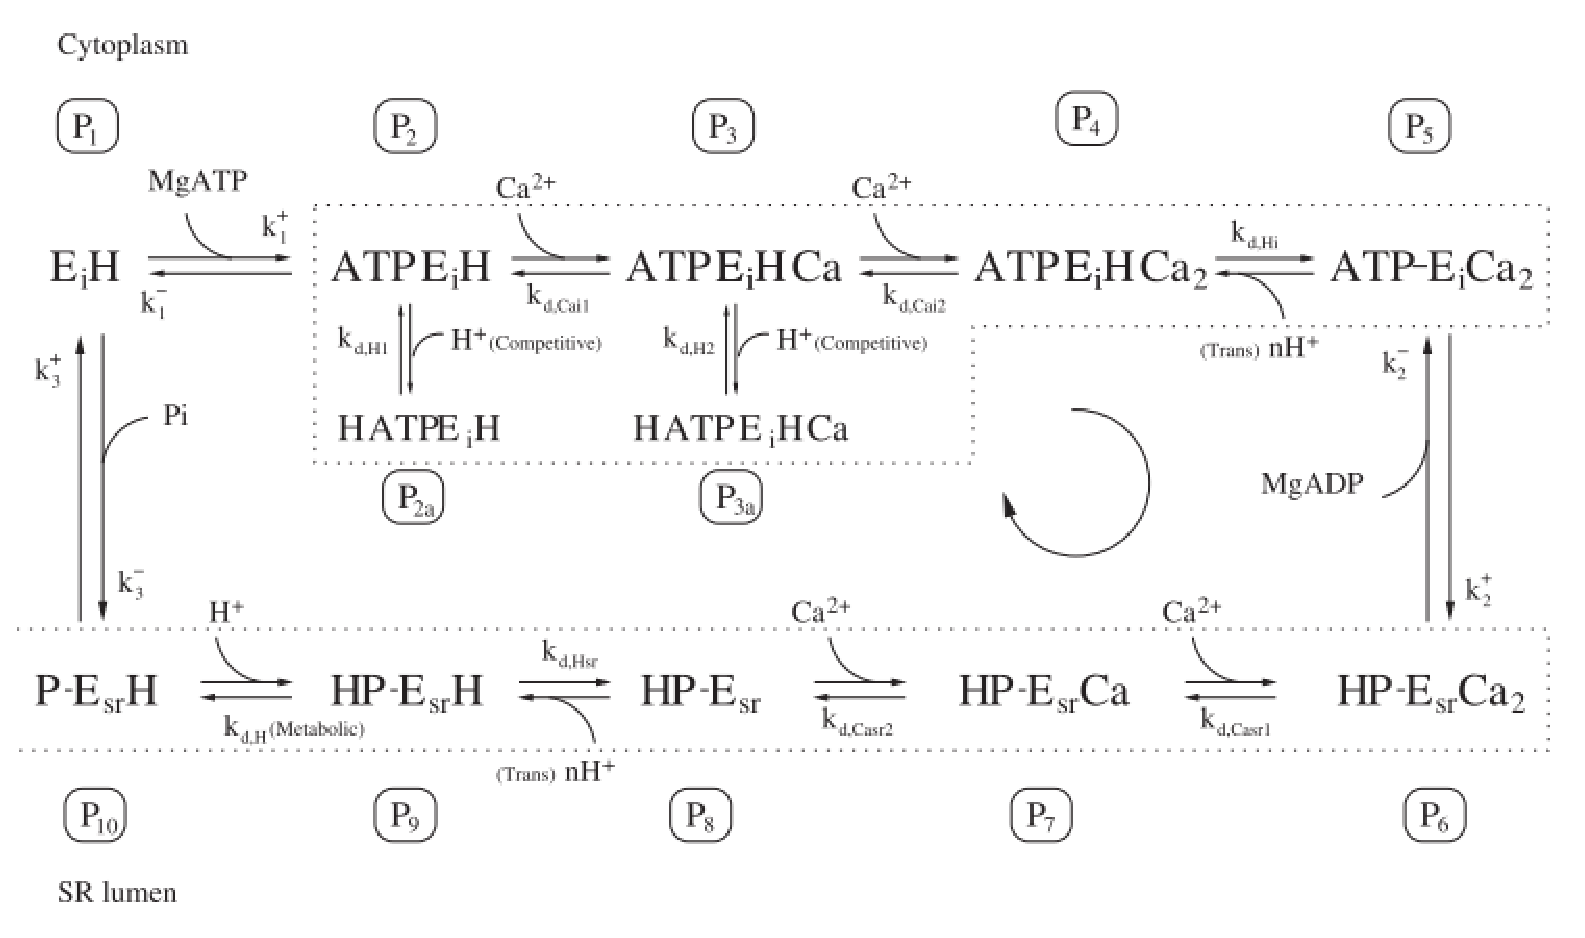
\includegraphics[height=7cm,
    angle=0]{./images/Tran_SERCA.eps}}
  \caption{12-state cardiac SERCA pump model. The box $P_n$ denotes
    the probability of being in a particular state $n$-th. The
    subscript $i$ and $sr$ is equivalent to 1 and 2 in E1-E2 notation,
    respectively}
  \label{fig:Tran_SERCA}
\end{figure}

\begin{equation}
  \label{eq:1267}
  \ce{2Ca_i^{2+} + MgATP + H2O <=> 2Ca^{2+}_{sr} + MgADP + Pi + H+}
\end{equation}

The reaction in eq.~\eqref{eq:1267} can be broken down into a number
of elementary reactions which is then mapped to a schematic diagram of
a 12-state model as given in Fig.~\ref{fig:Tran_SERCA}. The state-reduction
technique is based on \citep{smith2004} (Sect.\ref{sec:nak:-smith-crampin}). 

The flux is given by
\begin{equation}
J_\serca = 2 \times v_\cycle \times \rho_\sr \times A_\sr
\end{equation}
with $\rho_sr$ is the density of SERCA pump in the SR (unit: mole/cm$^2$; if
we map to (L cyt.) then we can use $\muM/$cm$^2$)); $A_\sr$ is the surface area
of the SR (unit: cm$^2$). Depending the number of states, $v_\cycle$ is
calculated using the associated formula (check the proper subsection).

\subsection{Parameter optimizations}
 \label{sec:param-estim}

Different datasets are used to constraint the parameters in the model. As these
data are measured at different temperatures, an no reliable values for Q10, the
authors determined to normalize them so that the maximum cycle rate is
$v_\cycle = 5$ (s$^{-1}$) at optimal conditions: 
\begin{verbatim}
Casr = 0
Cai = 10 uM
ATP = 5 mM
ADP = 0
Pi = 0
pH = 7.2
\end{verbatim}
These values were chosen based on maximal flux value of $v_\cycle=4.2$
(s$^{-1}$) obtained from intact rabbit myocytes at 22$^\circ$C. NOTE: Maximal
flux from canine and guinea pig ventricular myocytes (at 37$^\circ$C) are 5
(s$^{-1}$) and 7.5 (s$^{-1}$), respectively. 

% \subsection{Parameters estimation}
% \label{sec:param-estim}

Here, they choose all parameters, except $k^-_1$ which is determined based on
\begin{equation}
  \label{eq:1346}
  k^-_1 = \frac{k^+_1k^+_2k^+_3(K_{d,Casr})^2K_{d,Hi}K_{d,\H}}{k^-_2k^-_3(K_{d,Cai})^2K_{d,Hsr}\exp(\frac{dG_\ATP}{RT})}
\end{equation}
and then use the constraint in eq.~\eqref{eq:1283} to fit.

For the 3-state model, the parameters were estimated using particle
swarm optimization method. The solution then is used as the initial
guess in a Levenberg-Marquardt least-squares fitting procedure to
refine the solution. The fitting process can be carried out in Matlab
or COPASI software (free). 

\begin{verbatim}
k+1 = 25,900 [1/(mM.s)]
k+2 = 2540   [1/s]
k+3 = 20.5   [1/s]
k-1 = 2      [1/(mM.s)]
k-2 = 67,200 [1/(mM.s)]
k-3 = 149    [1/(mM.s)]
KdCai = 0.91 mM
KdCasr = 2.24mM
KdH1   = 1.09d-5 mM
KdHi   = 3.54d-8 mM^2
KdHsr  = 1.05d-8 mM^2
KdH    = 7.24d-5 mM
n      = 2 ! ion transport
\end{verbatim}


\subsection{Thermodynamics constraints}
\label{sec:therm-constr}

The free energy from the hydrolysis of a single ATP, $\Delta G_\MgATP$ to
transport $\Ca$ into the SR is coupled against the concentration gradient
$\Delta G_\SERCA$. So, the difference $\Delta G_\MgATP-\Delta G_\SERCA$ will
determine the direction of the pump when the myocyte is metabolically
compromised. The assumption is that for each ATP hydrolized, two $\Ca$ ions are
translocated.

\subsubsection{Ca/H countertransport}

There are two hypotheses of $\Ca$ binding: (1) partially cooperative, (2) fully
cooperative. The later one gives three fewer parameters to estimate. The authors
claimed that the residual is only 3\%, so they used the latter approach.
\textcolor{red}{The optimized parameters show a sigmoidal function of cytosolic
pCa} which is pH-dependent (i.e. shift to the right as pH decreased due to the
competitive binding of H+ to the $\Ca$-binding site when the site faces the
cytosol).

The SERCA pump flux exhibits a bell-shaped dependence on pH, with optimal flux
at pH $\approx 7.1$. The stoichiometry for the $\H$ binding was treated as a
parameter in the optimization, and is the most sensitive parameter. The chosen
value was n=2. This value governs the narrowness of the bell-shaped
relationship. 

\subsubsection{Metabolite dependence: Pi}

When Pi in the mM range, almost all SERCA enzymes are at phosphorylated state.
States P6-P10 are assumed to be in phosphorylated states.

\subsubsection{MgATP}

The free energy of ATp hydrolysis is reduced by increasing [Pi]. The pump stops
completely at the reversal point where the net free energy is zero. The rate at
which the SERCA pumps operate in reverse mode. Under normal $[\Ca]$ and pH
conditions, the maximal reverse mode $\frac{\alpha_1^- \alpha_3^-}{\alpha^+_1
+ \alpha_1^-+\alpha_3^-}$ is dominated by $\alpha^+_1$.


The free energy $\Delta G_\MgATP$ depends on the ratio of MgATP to its
hydrolysis product as
\begin{equation}
  \label{eq:1274}
  \Delta G_\MgATP = \Delta G_\MgATP^\circ + RT\ln \frac{[\MgADP][\Pi][\H]}{[\MgATP]}
\end{equation}
where $T$ is the temperature, $R$ is the universal gas constant,
$\Delta G^\circ_\MgATP$ is the free energy under standard condition. 
\begin{equation}
  \label{eq:1275}
  \Delta G^\circ_\MgATP = -RT\ln K_\MgATP = 11.9\;\; \text{kJ/mol}
\end{equation}
So, the energy required to move 2 $\Ca$ ions against the concentration
gradient is
\begin{equation}
  \label{eq:1276}
  \Delta G_\SERCA = 2RT\ln \frac{[\Ca]_\sr}{[\Ca]_i}
\end{equation}
In essence, the SERCA pump operate in the forward direction when the
net free energy $\Delta G_\MgATP + \Delta G_\SERCA < 0$. At
equilibrium, we have
\begin{equation}
  \label{eq:1280}
  \Delta G_\MgATP^\circ + RT\ln \frac{[\MgADP][\Pi][\H]}{[\MgATP]} +
  2RT\ln \frac{[\Ca]_\sr}{[\Ca]_i} = 0
\end{equation}
or
\begin{equation}
  \label{eq:1281}
  \Delta G_\MgATP^\circ + RT\ln
  \frac{[\MgADP][\Pi][\H][\Ca]^2_\sr}{[\MgATP][\Ca]_i^2}  = 0
\end{equation}
or
\begin{equation}
  \label{eq:1282}
  \frac{[\MgADP][\Pi][\H][\Ca]^2_\sr}{[\MgATP][\Ca]_i^2}  = \exp(-  \Delta G_\MgATP^\circ/(RT))
\end{equation}

Another constraint is the product of the forward transition rates is
equal to the product of the reversed transition rates
\begin{equation}
  \label{eq:1277}
  \prod k_i^+P_i = \prod k^-_i P_{i+1}
\end{equation}
where $P_i, P_{i+1}$ are fractional occupancies of adjacent
states. The rate constants are first-order.  If the transition
involves the binding/unbinding of an ion Y, then the expression is
written in the explicit form $k^+_i[Y]P_i$ and $k^+_i[Y]P_{i+1}$. The
fractional states $P_i$ are canceled out on both sides, leaving
\begin{equation}
  \label{eq:1278}
  \prod k_i^+ = \prod k^-_i 
\end{equation}
\textcolor{red}{which must hold whether or not the system in
  equilibrium}. Substituting the transition rates from the model, we
have
\begin{equation}
  \label{eq:1279}
  \frac{k^+_1k^+_2k^+_3K_{d,Casr1}K_{d,Casr2}K_{d,Hsr}K_{d,H}}{k^-_1k^-_2k^-_3K_{d,Cai1}K_{d,Cai2}K_{d,Hi}}
  = \frac{[\MgADP][\Pi][\H][\Ca]^2_\sr}{[\MgATP][\Ca]^2_\myo}
\end{equation}

Combining eq.~\eqref{eq:1282} and eq.~\eqref{eq:1279}, it yields a
constraint on the kinetic rate constants of the SERCA pump model
\begin{equation}
  \label{eq:1283}
  \frac{k^+_1k^+_2k^+_3K_{d,Casr1}K_{d,Casr2}K_{d,Hsr}K_{d,H}}{k^-_1k^-_2k^-_3K_{d,Cai1}K_{d,Cai2}K_{d,Hi}}
  =   \exp(-  \Delta G_\MgATP^\circ/(RT))
\end{equation}

\subsection{12-state}
\label{sec:12-state}

Here, the binding of $\Ca$ from the cytoplasm and SR lumen is modeled
as a partially cooperative mechanism, with different $K_d$ for the
first and second binding of $\Ca$.
\begin{itemize}
\item 2 for $\Ca$ in the cytoplasm, i.e. $P_2 \leftrightarrow P_3$, $P_3 \leftrightarrow P_4$
\item 2 for $\Ca$ in the SR lumen, i.e. $P_9 \leftrightarrow P_7$, $P_7 \leftrightarrow P_6$
\end{itemize}

Five $\H$ binding events:
\begin{itemize}
\item 2 for the competitive binding of $\H$ to the $\Ca$-binding site,
  i.e. $P_{2a}$ and $P_{3a}$. The competitive binding mechanism exist
  only when the $\Ca$-binding sites face the cytosol, and thus is not
  included in the model when it faces the SR lumen.

\item 2 for the binding of $\H$ involved in $\Ca/\H$
  counter-transport, $P_4 \leftrightarrow P5$ and $P_9 \leftrightarrow P_8$
\item one for the release of the metabolic $\H$. 
\end{itemize}

The conformational change between E1 and E2 occurs between $P_5 \leftrightarrow P_6$
(concomitant with MgADP release) and $P_{10} \leftrightarrow P_1$(concomitant with
Pi release). 

The stoichiometry of $\H$  binding in the SERCA model is an adjustable
parameter as it has been suggested that the number of $\H$ extruded
per cycle depends on pH.

\subsection{8-state}
\label{sec:8-state}

\begin{framed}
  The cooperative binding can be (1) {\it partially} or (2)
  {\it fully} cooperative. We have different binding constants for
  the first and second $\Ca$-binding. For partially cooperative, the
  second binding constant is set to a large value. For fully
  cooperative, the second binding instantaneous. 
\end{framed}

For fully cooperative, the second binding is assumed to be
instantaneous and thus the binding of the second $\Ca$ is assumed to
occur at the same time of the binding of the first $\Ca$. Thus, we
have a reduced 8-state model, Fig.~\ref{fig:Tran_8state}.

\begin{figure}[hbt]
  \centerline{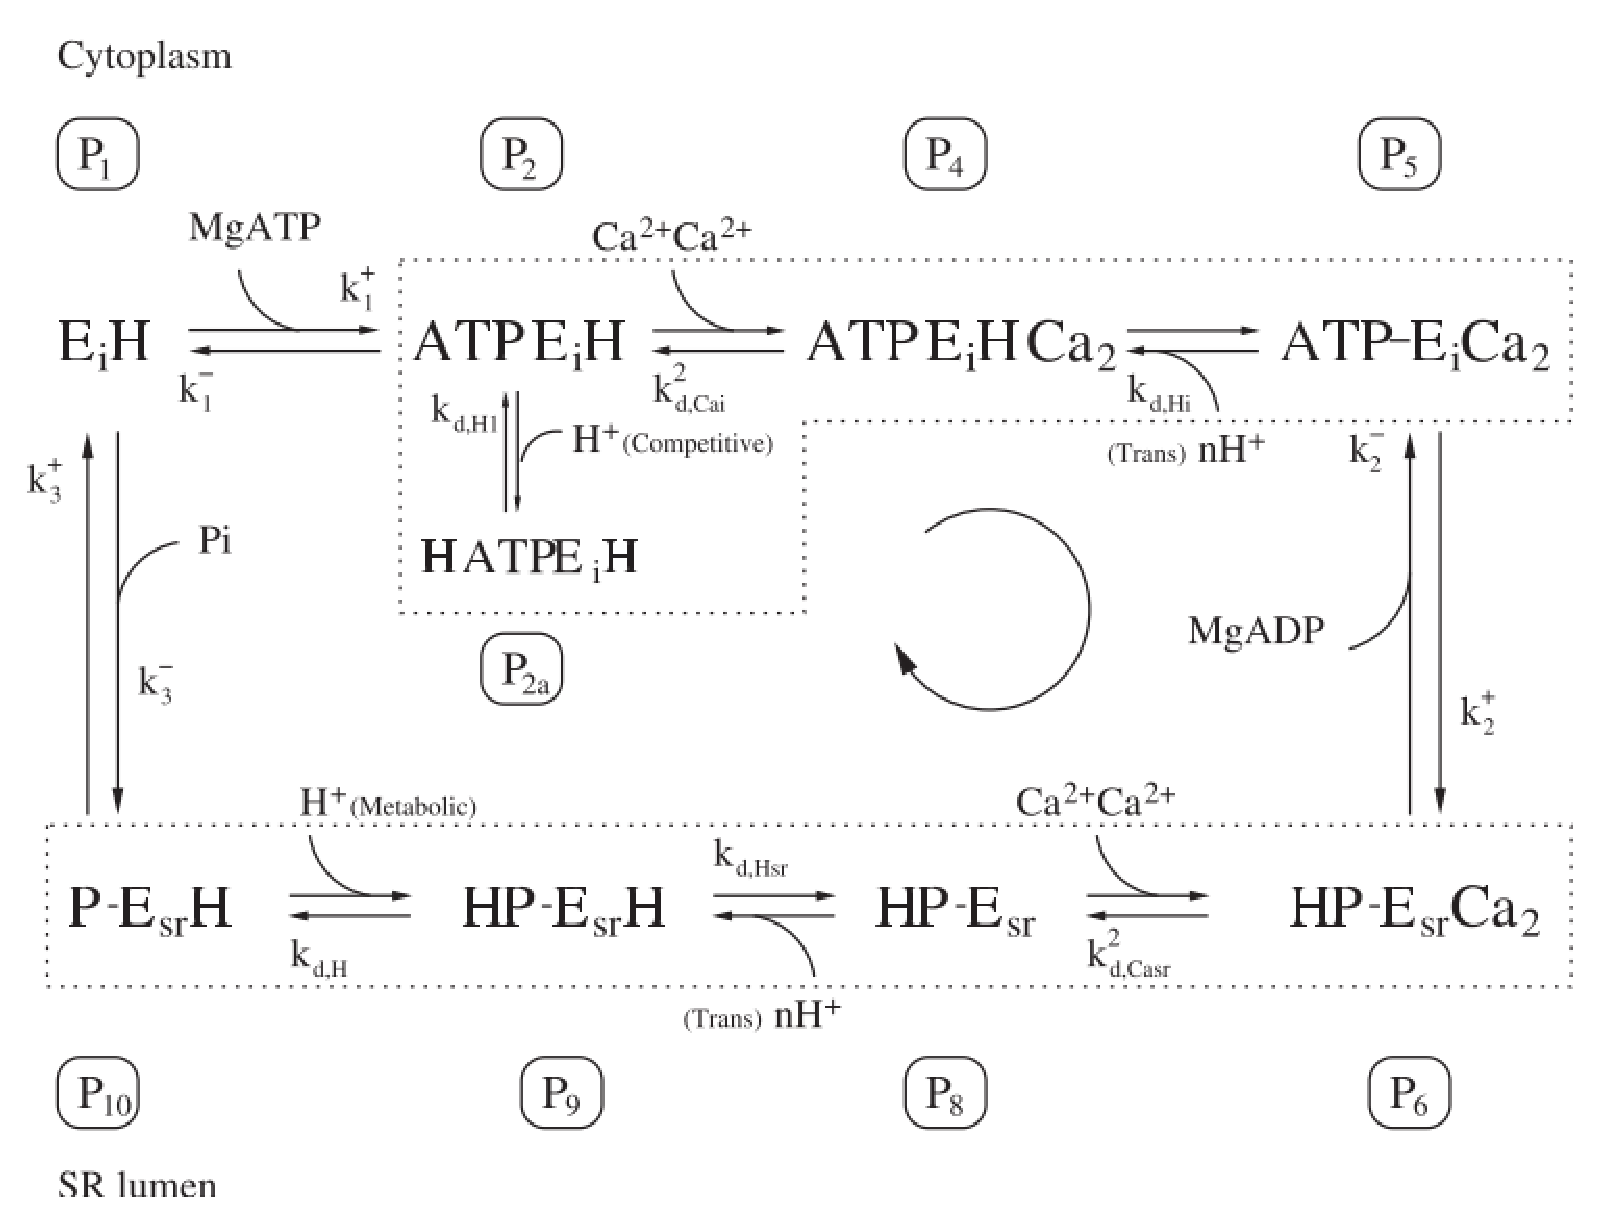
\includegraphics[height=5cm,
    angle=0]{./images/Tran_8state.eps}}
\caption{In fully cooperative, state $P_3$ and $P_{3a}$ no longer
  exist, as they quickly evolve into $P_4$. Similarly, $P_7$ and $P_6$
become a new state}
\label{fig:Tran_8state}
\end{figure}

\subsection{3-state}
\label{sec:3-state}

\textcolor{red}{In whole-cell simulation, the SERCA pump is assumed to
  operate at a kinetic steady-state}.
Thus, the 12-state model can be reduced to 3 states using rapid
equilibrium assumption of ion binding steps
(Sect.~\ref{sec:lump-rapid-equil} and
Sect.~\ref{sec:nak:-smith-crampin}).  Under the assumption that $\Ca$
and $H^+$ binding is faster the other metabolites, they assumed that
the entire $\Ca$ binding process (for both cytosol and SR lumen sides)
are faster than the subsequent conformational change of SERCA pumps.

As the native SR membrane is highly permeable to $\H$ and other
monovalent ions, the gradient is almost zero. Thus, $\H$ concentration
is assumed to be the same on both side of the SR.  Using
quasi-steady-state approximation, we have 3 states: $P_1$, $P_{2-5}$,
and $P_{6-10}$.
\begin{itemize}
\item 4 states from P2-P5 is grouped into one. The reason is that:
  Previous models assumed $\Ca$ bindings is fast for the first $\Ca$,
  and slow for the second one. Recent data suggested that
  conformational change after the first binding is minor (compared to
  E1-E2 conformational change)~\citep{tanford1987}. So, they assumed 2
  $\Ca$ binding for both cytosol and lumen-facing sites equilibrate
  rapidly comparison to E1-E2 conformational changes.

\item 5 states from P6-P10 is grouped into one. The justification is
  that MgADP and Pi partial reactions are slow, as these processes
  involves to the conformational change E1-E2, which is typically
  slow. In addition, the MgATP binding is modeled as slow since MgATP
  binding is shown to be a rate-limiting at very low concentrations
  (i.e. $\mu$M range)~\citep{mintz1997}.

\end{itemize}


\begin{figure}[hbt]
  \centerline{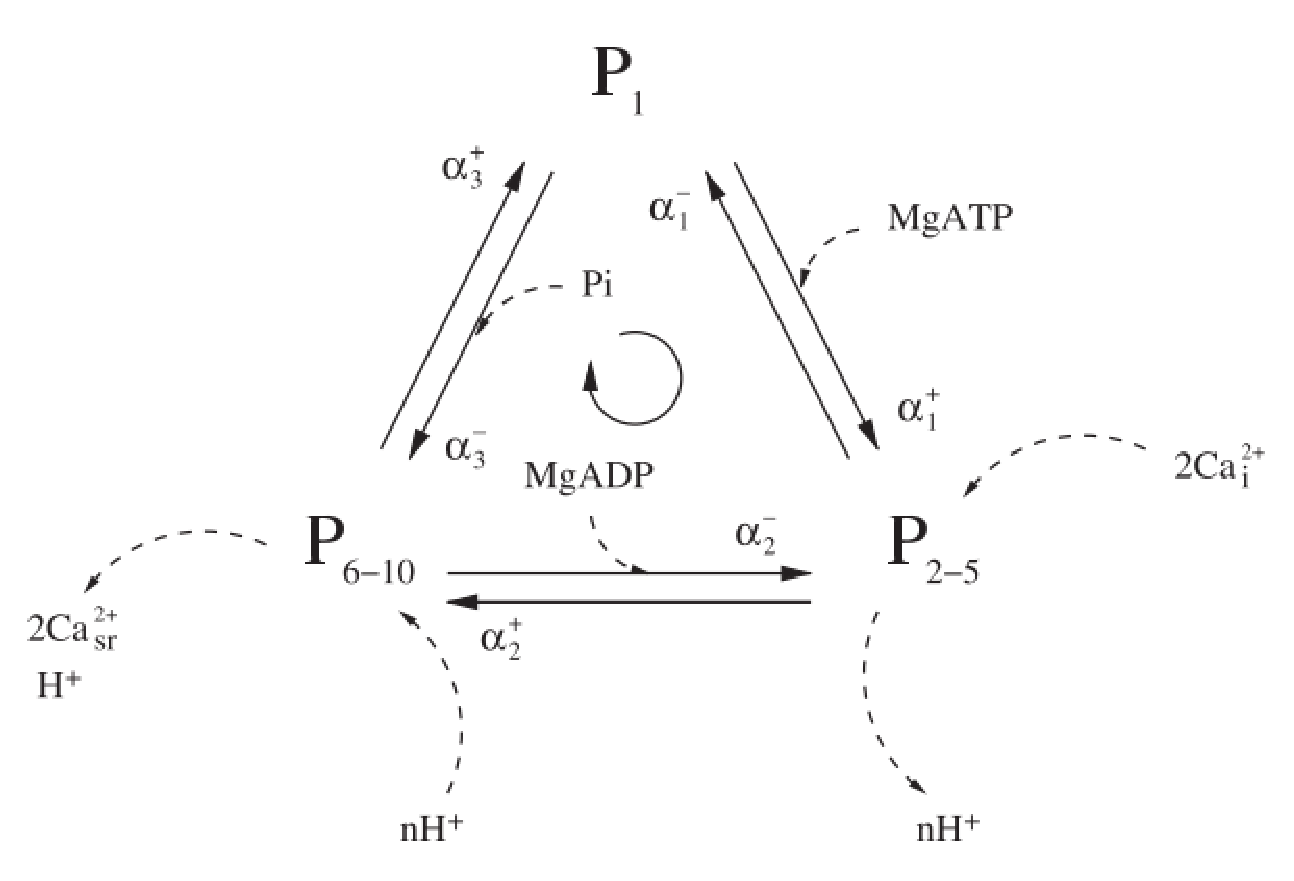
\includegraphics[height=5cm,
    angle=0]{./images/Tran_3state.eps}}
\caption{A simplified 3-state model with apparent rate constants
  $\alpha_i^\pm, i=1,2,3$)}
\label{fig:Tran_3state}
\end{figure}  
  
So, the steady-state of the flux is solved using diagram
method,
with the {\it clockwise cycle} rate per pump at steady-state is
\begin{equation}
  \label{eq:987}
  v_\cycle = \frac{\alpha^+_1\alpha^+_2\alpha^+_3-\alpha^-_1\alpha^-_2\alpha^-_3}{\sum_3} \;\;\; (s^{-1})
\end{equation}
with $\sum_3$ is the sum of 9 positive product terms $\alpha$.

Finally, to integrate in the whole-cell model, the whole-cell pump
flux is given by
\begin{equation}
  \label{eq:988}
  J_\serca = 2v_\cycle. \rho_\sr .A_\sr \;\;\; (\text{mol.s}^{-1})
\end{equation}
the factor 2 means 2 $\Ca$ ions are transported in each cycle.
$\rho_{sr}$ is the density of SERCA pump per unit of membrane,
$A_{sr}$ is the surface area of the SR membrane.

\begin{framed}
  In temporal-spatial whole-cell modeling, we need to divide $A_\sr$
  into the correct area in each grid element. 
\end{framed}

The parameters in the 3-state was optimized using particle swamp
method (COPASI software). 

\subsection{2-state}
\label{sec:2-state}

Under physiological condition, or even ischemia condition, MgATP
concentration is still high (mM range), e.g. in healthy myocyte $\sim$
5mM can drop to 50\% during ischemia, so the binding of MgATP can be
considered fast and instantaneously reach equilibrium. 

So, under physiological, or even in ischemia condition, the 3-state
model can be simplified into a 2-state model,
Fig.~\ref{fig:Tran_2state}.

\begin{figure}[hbt]
  \centerline{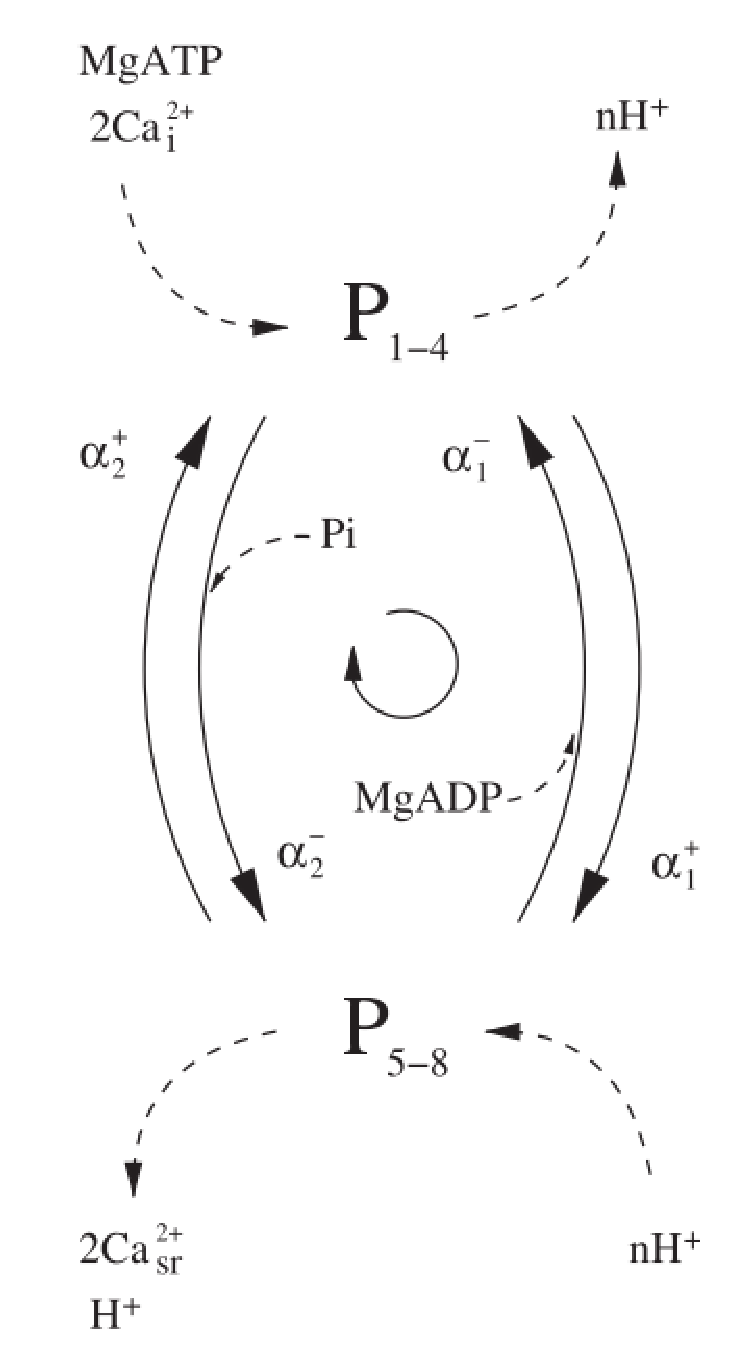
\includegraphics[height=6cm,
    angle=0]{./images/Tran_2state.eps}}
\caption{Using rapid equilibrium of MgATP binding, the model is
  simplified to 2 states}
\label{fig:Tran_2state}
\end{figure}

The cycling rate [1/sec] is given as
\begin{equation}
  \label{eq:1273}
  v_\cycle = \frac{\alpha^+_1\alpha^+_2-\alpha^-_1\alpha^-_2}{\sum_2}
\end{equation}
with $\sum_2 = \alpha^+_1+\alpha^+_2+\alpha^-_1+\alpha^-_2$, and the
forward rate constant
\begin{equation}
  \label{eq:1268}
  \alpha_1^+ = \frac{k^+_2 \MgtATP.\ca_i^2}{\MgtATP.\ca_i^2 + \tH_i(1+\MgtATP(1+\tH_1+\ca_i^2))}
\end{equation}
\begin{equation}
  \label{eq:1269}
  \alpha_2^+ = \frac{k^+_3\tH_\sr}{\tH_\sr(1+\tH)+\tH(1+\ca^2_\sr)}
\end{equation}
and backward rate constants
\begin{equation}
  \label{eq:1270}
  \alpha^-_1 =  = \frac{k^-_2 [\MgADP]\ca^2_\sr\tH}{\tH_\sr(1+\tH)+\tH(1+\ca_\sr^2)}
\end{equation}
\begin{equation}
  \label{eq:1271}
  \alpha_2^-=\frac{k^-_3[\Pi]\tH_i}{\MgtATP.\ca^2_i + \tH_i(1+\MgtATP(1+~\H_1+\ca^2_i))}
\end{equation}
where the unitless variables are
\begin{equation}
  \label{eq:1284}
  \begin{array}{cc}
    \ca_i = \frac{[\Ca]_\myo}{K_{d,Cai}} &
    \tH_i = \frac{[\H]}{K_{d,Hi}} \\
    \tH_1=\frac{[\H]}{K_{d,H1}} &
    \ca_\sr = \frac{[\Ca]_\sr}{K_{d,Casr}} \\
    \tH_\sr = \frac{[H+]}{K_{d,Hsr}} &
    \tH = \frac{[\H]}{K_{d,H}}
  \end{array}
\end{equation}
with $[\H]=???$, and
\begin{equation}
  \label{eq:1272}
  \begin{split}
    \MgtATP = \frac{[\MgATP]}{K_{d,ATP}} \\
    K_{d,ATP} = \frac{k^-_1}{k^+_1} =
    \frac{k^+_2k^+_3K^2_{d,Casr}K_{d,Hi}K_{d,H}}{k^-_2k^-_3K^2_{d,Cai}K_{d,Hsr}e^{\Delta G^o_{MgATP}/(RT)}}
  \end{split}
\end{equation}
with $\Delta G^o=11.9$kJ/mol, R=8.314 J/K/mol, T is temperature
[K]. The second equation is derived from eq.~\eqref{eq:1283}.

\subsection{Data analysis}
\label{sec:data-analysis-2}

The increase in $[\Ca]_\sr$ leads to a decrease in pump rate until a
reversal point is reached where the pump begin to operate in the
reverse mode. This reverse mode is predicted to start at
$[\MgATP]=5$mM which is almost negligible over either the
physiological or ischemic range of $[\Pi]$.
\begin{itemize}
\item $[\ADP]=36.3\mu$M, pH=7, $[\Ca]_i=150$nM. 
\end{itemize}

SERCA flux is a sigmoidal function of cytosolic pCA. This sigmoidal
function is pH-dependent and shift progressively to the right
(i.e. increase $K_m$) as pH decreases. This is due to the fact that
low pH, i.e. more $\H$ and more competitive in binding with $\Ca$ on
cytosolic side. At a normal pH=7, $K_m$ for the $\Ca$ flux curve is
0.26$\mu$M, similar to the parameters employed in the reverse model
by~\citep{shannon2000rms}.

SERCA flux also exhibits a bell-shaped function of pH, and operate
optimally at pH$\sim$7.1.

SERCA flux increases with increasing [MgATP] and reaches a saturating
value that is dependent on the [MgADP].

There are evidence that the coupling ratio of $\Ca$ transport can be
lower than 2 in the absence of oxalate (a chelator of luminal
$\Ca$)~\citep{yu1995}, causing a high level of lumenal $\Ca$
concentration. However, under physiological conditions in the beating
heart, it's reasonable to assume the lumenal $\Ca$ levels do not
approach such a high range and therefore the transport of $\Ca$ can be
assumed to tightly couple to the hydrolysis of ATP with the
stoichiometric ratio of 2..


%%% Local Variables: 
%%% mode: latex
%%% TeX-master: "mainfile"
%%% End: 
